\chapter{Results}

This chapter reports the empirical findings of the experimental programme. Section 4.1 characterises the three LLM judges at baseline, before any defence is applied. Section 4.2 reports the statistical pre-filter as a passage-level classifier. Section 4.3 reports the LLM pre-filter (Mistral) as a triplet-level classifier. Section 4.4 is the central section of the chapter: it measures how each pre-filter affects judge reliability end-to-end, using a labelling convention that reflects what the judge actually sees after filtering. Section 4.5 audits what each filter did at the passage level and surfaces a collateral-damage finding that explains part of the end-to-end behaviour. Section 4.6 reports the justification analysis. Section 4.7 reports the multi-judge disagreement analysis. Section 4.8 summarises.

\section{Baseline Judge Characterisation}

We score the full Poisoned Evaluation Dataset with each of the three judges (GPT-5.4-nano, Gemma-4-26B-A4B-IT, DeepSeek-V3.2) without any filter applied. The results establish how vulnerable each judge is to corpus poisoning before any defence is in place, and they surface qualitatively different scoring behaviours that shape every analysis that follows.

\subsection{Cross-judge baseline failure rates}

A note on terminology before the numbers. Throughout this chapter, two related but distinct quantities are reported: the False Positive Rate (the fraction of poisoned triplets the judge scores at or above 0.5) and the mean RAGAS score on a particular subset. Higher values of either quantity, when computed on a poisoned subset, indicate judge failure rather than judge success - the judge is assigning faithful or relevant labels to context that is by construction corrupted. This convention applies uniformly across the faithfulness, context relevance, and answer relevance dimensions.

Baseline False Positive Rates differ substantially across judges. Table~\ref{tab:baseline-fpr} reports FPR on the originally-poisoned subset for all three RAGAS dimensions.

\begin{table}[H]
\centering
\small
\resizebox{\textwidth}{!}{%
\begin{tabular}{llll}
\toprule
Judge & Faithfulness FPR & Context Relevance FPR & Answer Relevance FPR \\
\midrule
GPT-5.4-nano & 0.555 & 0.720 & 0.727 \\
Gemma-4-26B-A4B-IT & 0.699 & 0.860 & 0.889 \\
DeepSeek-V3.2 & 0.412 & 0.326 & 0.652 \\
\bottomrule
\end{tabular}
}
\caption{Baseline FPR across the three RAGAS dimensions (n=1,200 originally-poisoned triplets per judge per metric, except Gemma where two API failures reduce n to 1,199).}
\label{tab:baseline-fpr}
\end{table}

The headline numbers tell three different stories. DeepSeek is the strictest of the three on faithfulness and context relevance; it scores roughly 41\% of poisoned triplets as faithful and 33\% as having relevant context. Gemma is the most lenient by a wide margin, scoring more than 86\% of poisoned triplets as having relevant context. GPT sits in the middle on faithfulness but produces a high context relevance FPR (0.720).

Answer relevance FPR is the highest of the three RAGAS dimensions for every judge. This is structural rather than a sign of judge failure: the answer in our triplets is the HotpotQA ground-truth answer, which is genuinely relevant to the question regardless of what the context contains. We retain answer relevance throughout the analysis as a methodological control. It shows what a judge's behaviour looks like on a metric that is in principle insensitive to context corruption, and it provides a reference point against which faithfulness and context relevance behaviour can be compared.

\subsection{Three calibration regimes}

The three judges occupy distinct calibration regimes that emerge from their score distributions on faithfulness (Figure~\ref{fig:baseline-calibration}). The differences are not subtle.

\begin{figure}[H]
\centering
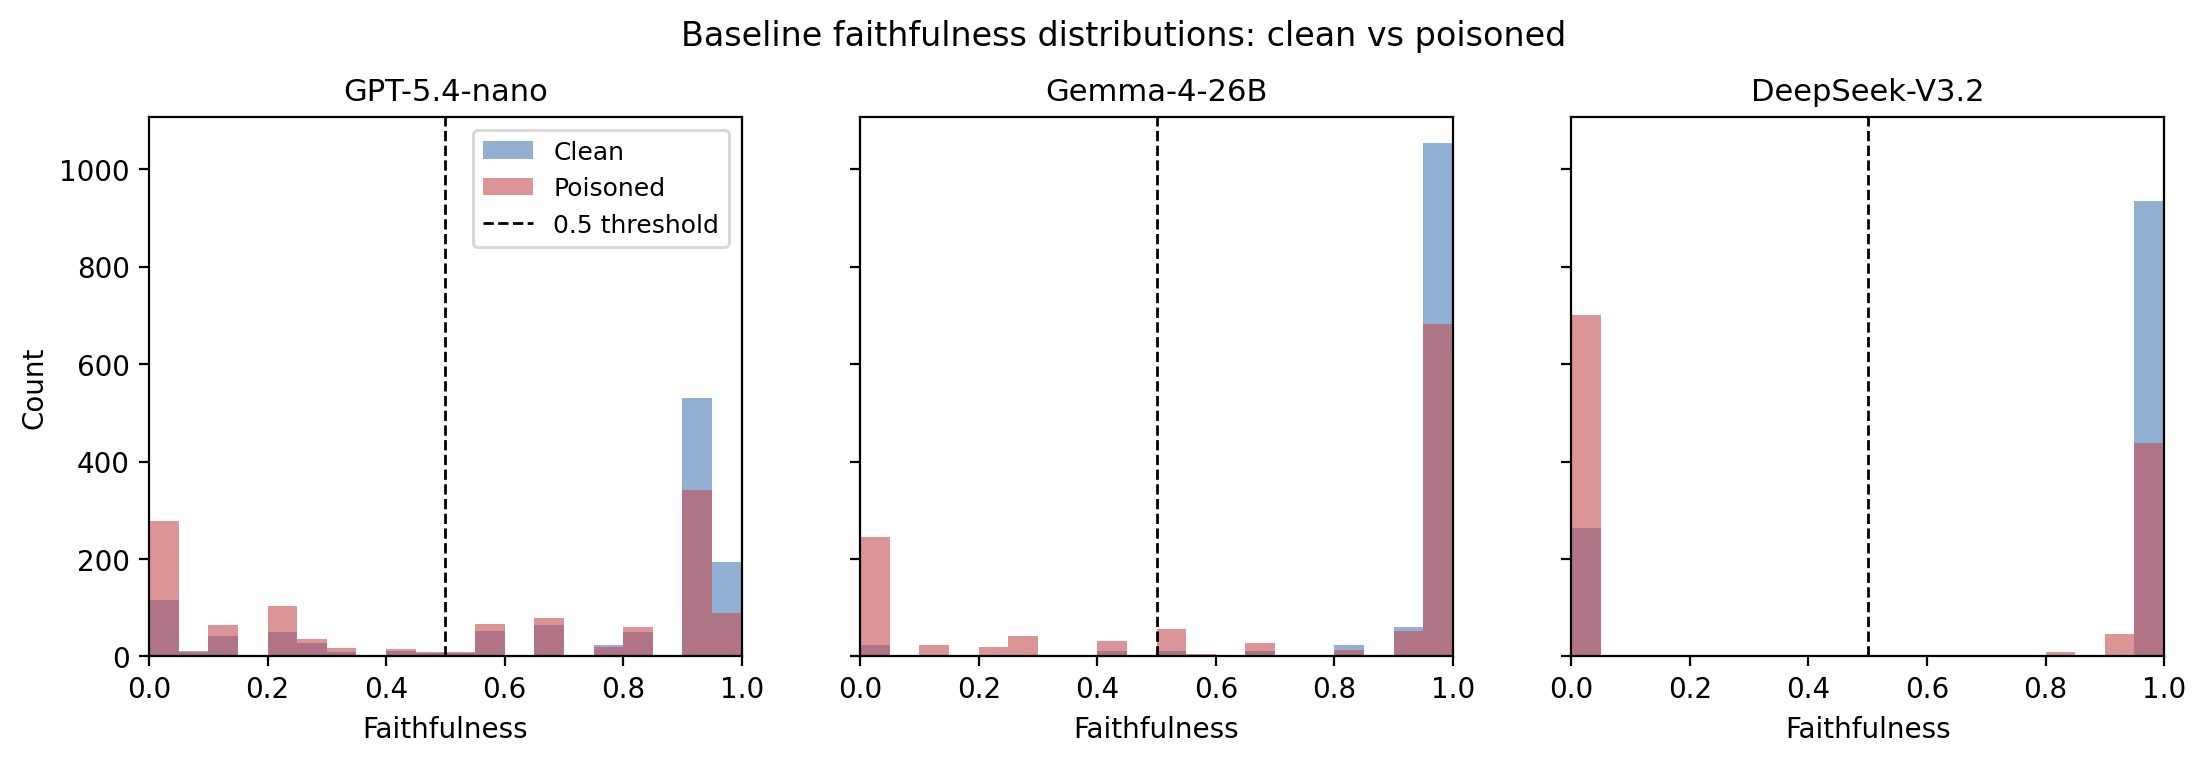
\includegraphics[width=0.95\textwidth]{../exports/figures/fig01_baseline_calibration.png}
\caption{Baseline faithfulness score distributions for clean and poisoned triplets, shown separately for each judge. The dashed vertical line marks the 0.5 threshold used to convert scores into false-positive decisions.}
\label{fig:baseline-calibration}
\end{figure}

GPT produces a continuous distribution. Scores spread across the full [0, 1] interval, with 30.3\% landing in the middle range (0.1 to 0.9 exclusive), 21.5\% at or below 0.1, and 48.2\% at or above 0.9. The judge expresses graded confidence and a threshold of 0.5 is one of many reasonable choices for binarising its output. The behaviour around the threshold is not bimodal, though the distribution leans toward high scores.

Gemma exhibits extreme leniency. About 77.1\% of faithfulness scores fall at 0.9 or above, and only 10.7\% land in the middle range. The judge defaults to high faithfulness scores and reserves low scores for the most extreme cases. This is the source of Gemma's high baseline FPR: when the default verdict is "faithful", poisoning has to be glaring to overcome that prior.

DeepSeek is near-binary. About 99.4\% of scores cluster at the extremes (≤0.1 or ≥0.9), with only 0.6\% in the middle range. The judge effectively makes a binary decision and reports it as a near-extreme number. The threshold of 0.5 is essentially a formality for this judge; the meaningful question is which of the two attractors a given triplet falls into.

These calibration regimes matter for two reasons that recur through the chapter. First, they constrain which mitigation strategies are even applicable. A continuous-scoring judge supports confidence-abstention strategies because there is a meaningful uncertainty band to abstain on. A near-binary judge does not. Second, the calibration regimes interact non-trivially with attack type, as the next subsection shows.

A note on terminology: throughout this chapter we use "calibration regime" specifically to refer to the \textit{shape} of the score distribution (continuous, near-binary, extreme-leniency). This is a structural property of how a judge maps internal confidence to a [0, 1] output. It is distinct from the stronger sense of "calibration" used in probabilistic forecasting, where a well-calibrated predictor's confidence values match empirical accuracy on held-out data. Validating the three judges' calibration in that stronger sense would require a human-annotated ground truth, which we do not have for this dataset; we treat that as a limitation in Section 5.5.

\subsection{Cross-judge divergence on PoisonedRAG-style attacks}

The three injection types do not affect the three judges in the same way. Table~\ref{tab:baseline-fpr-injection} shows poisoned-set faithfulness FPR by judge and injection type.

\begin{table}[H]
\centering
\begin{tabular}{llll}
\toprule
Judge & Random noise & Adversarial fact & PoisonedRAG-style \\
\midrule
GPT-5.4-nano & 0.490 & 0.560 & 0.615 \\
Gemma-4-26B-A4B-IT & 0.570 & 0.620 & 0.907 \\
DeepSeek-V3.2 & 0.465 & 0.398 & 0.375 \\
\bottomrule
\end{tabular}
\caption{Baseline faithfulness FPR by injection type, per judge. Each cell uses n=400 originally-poisoned triplets.}
\label{tab:baseline-fpr-injection}
\end{table}

The cross-judge ordering reverses on PoisonedRAG-style. For GPT and Gemma, PoisonedRAG-style is the hardest of the three injection types to detect; their FPRs climb to 0.615 and 0.907 respectively. For DeepSeek, PoisonedRAG-style is the easiest of the three, with FPR dropping to 0.375. Gemma's FPR on PoisonedRAG-style is more than double DeepSeek's on the same attack class.

The reversal is striking and worth interpreting carefully. PoisonedRAG-style is the most adversarial of the three classes by construction. The retrieval sub-text guarantees the malicious passage will be retrieved, and the generation sub-text is engineered to support a target wrong answer that contradicts the ground-truth answer. The fact that GPT and Gemma find this hardest reflects what the attack is designed to do: produce content that looks topically coherent and factually plausible while steering toward the wrong answer.

DeepSeek's response is different in kind, and the cleanest interpretation we can offer connects this to its calibration regime. The near-binary scoring style means DeepSeek is not weighing graded evidence; it is making a categorical judgement. PoisonedRAG-style triplets contain an internal contradiction (the malicious passage supports an answer that contradicts the ground-truth answer in the triplet's answer slot), and DeepSeek's scoring style picks up on that contradiction reliably while the continuous-scoring judges weight the topical fluency of the malicious passage more heavily than the contradiction. We offer this as the most plausible mechanism consistent with our data; we cannot rule out alternative explanations such as DeepSeek's training distribution containing more contradiction-detection examples or its system-prompt sensitivity differing from the others. The directional reversal is robust; the mechanism behind it is partially speculative.

Within our three-judge panel, scoring strategy appears to matter at least as much as judge size or training compute for robustness to corpus poisoning. The three judges respond differently to the most sophisticated attack class, and the differences within our panel are not explained by raw model capacity or simple bias correction. Whether the same observation holds across a larger panel - particularly one that includes reasoning models or frontier-tier judges - is an empirical question we cannot answer with three judges; we treat the claim as suggested by our data, not established by it.

\subsection{Noise level sensitivity}

Within each injection type, FPR varies with noise level (the proportion of context passages replaced). The pattern is broadly monotonic: higher noise levels are easier to detect for all three judges. At noise level 0.2, GPT's faithfulness FPR is 0.700; at noise level 0.8 it falls to 0.423. Gemma's drops from 0.850 to 0.555 across the same range. DeepSeek's falls most steeply, from 0.597 to 0.233.

The direction matches intuition. When more of the context is corrupted, the corruption becomes harder to ignore. The implication for the security narrative is mixed. Low-noise attacks (where most of the context is still legitimate) are the harder threat because the judges are more vulnerable to them. The structural failure cases that drive the highest FPRs (PoisonedRAG-style on GPT and Gemma) are not strongly noise-dependent; subtle attacks succeed at high baseline rates regardless of how much surrounding noise is present.

The noise-level pattern reverses partially after filtering, which we examine in Section 4.4.

\section{Statistical Pre-filter as a Classifier}

Section 4.1 established that judges are vulnerable. We now turn to the first proposed mitigation: a multi-signal statistical pre-filter that scores each retrieved passage and removes those flagged as poisoned. The filter is evaluated as a binary passage-level classifier on the held-out test split of the Poisoned Evaluation Dataset.

\subsection{Headline performance}

The filter performs well. On 5,119 test-split passages (1,155 poisoned, 3,964 clean), it achieves precision 0.955, recall 0.904, and F1 of 0.929. The clean false-positive rate is 0.012 - clean passages are essentially never wrongly flagged.

\begin{table}[H]
\centering
\begin{tabular}{ll}
\toprule
Metric & Value \\
\midrule
Test-set F1 & 0.929 \\
Precision & 0.955 \\
Recall & 0.904 \\
Clean false-positive rate & 0.012 \\
\bottomrule
\end{tabular}
\caption{Statistical pre-filter performance on the held-out test split (5,119 passages).}
\label{tab:stat-filter-performance}
\end{table}

These are strong numbers in absolute terms. The filter is highly precise: when it flags a passage as poisoned, it is right about 95.5\% of the time. The clean-FPR of 0.012 is operationally meaningful - clean passages are essentially never wrongly removed, which means the filter does not aggressively reject legitimate retrieved content.

\subsection{Recall by attack type}

The filter's behaviour varies by injection type. Table~\ref{tab:stat-filter-by-injection} reports per-attack-type performance on the test split.

\begin{table}[H]
\centering
\small
\resizebox{\textwidth}{!}{%
\begin{tabular}{lllllll}
\toprule
Injection type & n test passages & n poisoned & Precision & Recall & F1 & Clean FPR \\
\midrule
Random noise & 1,595 & 392 & 0.954 & 0.903 & 0.928 & 0.014 \\
Adversarial fact & 1,590 & 389 & 0.955 & 0.812 & 0.878 & 0.013 \\
PoisonedRAG-style & 1,934 & 374 & 0.957 & 1.000 & 0.978 & 0.011 \\
\bottomrule
\end{tabular}
}
\caption{Statistical filter classifier performance per injection type, test split.}
\label{tab:stat-filter-by-injection}
\end{table}

The filter performs well across all three attack types. Recall is highest on the most adversarial class (PoisonedRAG-style at 1.000) and lowest on the middle class (adversarial fact at 0.812). The PoisonedRAG-style result is striking: the filter catches every poisoned PoisonedRAG passage in the test set. The combined signal set evidently captures structural artefacts of the attack reliably; identifying which individual signals carry the most weight in this regime is examined in Section 4.2.3 below.

The adversarial fact class is the hardest because the manipulation is at the factual level, not at the surface or structural level. The injected passage is fluent, topically aligned with the question, and embedding-similar to the original passage it replaces. The filter must rely on the DeBERTa classifier (Signal 3) and answer span recall (Signal 4) to catch these cases, and not all of them carry strong enough signal for the classifier to flag.

\subsection{Per-signal contribution and classifier backbone}

A per-signal ablation removes one signal at a time and recomputes pipeline F1. The DeBERTa classifier (Signal 3) is the largest single contributor: removing it drops F1 by approximately 0.030. The cross-encoder (Signal 5) contributes roughly 0.029 and answer span recall (Signal 4) contributes roughly 0.018. The embedding cosine and entropy signals contribute negligibly to aggregate F1 in this ablation; removing either changes overall F1 by less than 0.001.

The per-injection ablation breakdown (Appendix D) shows that the per-signal contributions vary somewhat by attack type but no single signal dominates PoisonedRAG-style detection in isolation. The combined signal set, taken together, achieves the high test-split PoisonedRAG-style recall reported in Table~\ref{tab:stat-filter-by-injection} - but the ablation does not identify a single removable signal whose absence collapses that recall. The headline interpretation is that the multi-signal aggregation is genuinely doing aggregate work; the filter is not reducible to any one of its inputs.

The classifier backbone comparison (DeBERTa-v3-small vs RoBERTa-base, both fine-tuned on the same training split with matched hyperparameters) shows the two architectures essentially tied at validation F1 of 0.7215 and 0.7202. Either backbone produces a usable filter; the choice between them is not load-bearing for the headline results. Detailed ablation tables are reported in Appendix D.

The headline of Section 4.2 is straightforward: the statistical filter is a strong classifier, with high precision (0.955) and high recall (0.904) on the held-out test set. Three of its five signals (DeBERTa, cross-encoder, answer span recall) carry the discriminative weight in aggregate F1. The filter performs particularly well on PoisonedRAG-style attacks at the test-set operating point.

\section{LLM Pre-filter (Mistral) as a Classifier}

The second pre-filter strategy uses \texttt{mistral-small-latest} as a triplet-level classifier. Section 3.4.5 set out the rationale: a triplet-level operating mode (the filter sees all retrieved passages at once and gives a single verdict) and a deliberate cross-architecture choice (Mistral is outside both the poison-generation family and all three judge families).

\subsection{Headline performance}

\begin{table}[H]
\centering
\begin{tabular}{ll}
\toprule
Metric & Value \\
\midrule
Triplets evaluated & 2,400 \\
Mistral recall on poisoned triplets & 0.505 \\
Precision & 0.744 \\
F1 & 0.601 \\
Clean false-positive rate & 0.174 \\
\bottomrule
\end{tabular}
\caption{Mistral triplet-level filter performance.}
\label{tab:mistral-filter-performance}
\end{table}

Mistral catches just over half of the poisoned triplets, with a clean-FPR of 0.174 - about one in six clean triplets is wrongly flagged. The trade-off relative to the statistical filter is sharp: lower recall (0.505 vs 0.904), substantially higher clean-FPR (0.174 vs 0.012), at a coarser granularity (whole-triplet rejection rather than per-passage removal).

\subsection{Strong asymmetry by attack type}

Mistral's per-attack-type behaviour reveals a sharp asymmetry that the statistical filter does not exhibit.

\begin{table}[H]
\centering
\small
\resizebox{\textwidth}{!}{%
\begin{tabular}{lllllll}
\toprule
Injection type & n poisoned & n clean & Precision & Recall & F1 & Clean FPR \\
\midrule
Random noise & 400 & 400 & 0.438 & 0.140 & 0.212 & 0.180 \\
Adversarial fact & 400 & 400 & 0.775 & 0.610 & 0.683 & 0.178 \\
PoisonedRAG-style & 400 & 400 & 0.823 & 0.765 & 0.793 & 0.165 \\
\bottomrule
\end{tabular}
}
\caption{Mistral triplet-level performance by injection type.}
\label{tab:mistral-filter-by-injection}
\end{table}

Mistral catches 76.5\% of PoisonedRAG-style triplets but only 14.0\% of random-noise triplets. The recall asymmetry is more than five-to-one. This is the exact opposite profile from the statistical filter, which has its strongest recall on PoisonedRAG-style (1.000) and weakest on adversarial fact (0.812).

The two filters detect partially complementary phenomena. The statistical filter exploits structural artefacts of the attacks (retrieval-optimised embeddings, classifier-detectable text patterns, missing answer tokens). Mistral judges the triplet as a whole and reasons about cross-passage consistency. PoisonedRAG-style attacks are easy for Mistral because the malicious passage explicitly contradicts the supporting passages in a way that a cross-passage reading can detect. Random-noise attacks are hard for Mistral because the noise passages are irrelevant rather than contradictory; they do not produce the kind of internal inconsistency Mistral can flag from a holistic reading.

The complementarity has implications for hybrid filter design that we return to in Section 5.4.

\section{End-to-End Effect of Filtering on Judge Reliability}

This is the central section of the chapter. Sections 4.2 and 4.3 measured each filter as a classifier in isolation. The question that matters for production deployment is different: when a filter sits between the retriever and the judge, does the judge become more reliable? The answer is more nuanced than the standalone classifier metrics suggest, and reaching it requires care about what we are measuring.

\subsection{Defining what "post-filter FPR" should measure}

The naive post-filter FPR computation takes every triplet that was originally poisoned and asks how often the judge scores it as faithful after filtering. This computation has a conceptual problem. The statistical filter modifies content. After it runs, a triplet that was originally poisoned may have only had distractor passages perturbed (the supporting passages survived the attack) or may have had supporting passages overwritten (the supporting passages were killed). The two cases look very different to the judge, and aggregating them under a single "originally poisoned" label hides what is actually happening.

We therefore decompose the originally-poisoned subset into two categories using the explicit per-passage poisoning indices recorded at construction time:

\begin{itemize}
  \item \textbf{True}: the originally-supporting passages were among the poisoned ones (the attack hit the support and the judge faces concentrated poison at evaluation time).
  \item \textbf{Survived}: the originally-supporting passages were not among the poisoned ones (the attack hit only distractor positions, or augmented the context additively, leaving clean support intact).
\end{itemize}

The decomposition has a structural consequence specific to our injection design. Type 1 (random noise) and Type 2 (adversarial fact rewriting) overwrite passages in place: the random sample of replacement positions can either hit or miss the supporting passages, producing a mixture of True and Survived triplets per injection type. Type 3 (PoisonedRAG-style) operates additively: malicious passages are inserted alongside the original passages without overwriting any of them. As a structural consequence of additive injection, Type 3 triplets are always in the Survived category - the supporting passages are present in every Type 3 poisoned context, simply alongside the inserted malicious content. This means the True subset is composed entirely of Type 1 and Type 2 triplets, while the Survived subset contains a mixture of Type 1, Type 2 (where the random replacement happened to miss support), and all of Type 3.

This asymmetry is not a limitation of the analysis but a consequence of how the attacks work: PoisonedRAG-style is by design a poison-augmentation attack rather than a replacement attack, so its end-to-end behaviour is captured in the Survived subset. We report behaviour on each subset separately. Comparing baseline-True to postfilter-True isolates how filtering changes the judge's response to the worst case (concentrated poison after support has been overwritten). Comparing baseline-Survived to postfilter-Survived isolates how filtering changes the judge's response to the case where support is intact alongside poison.

The split is computed by exact-title matching against per-question passage title lists rather than by substring search. Of 1,200 originally-poisoned triplets, 576 fall into the True category (288 random\_noise + 288 adversarial\_fact + 0 poisonedrag\_style) and 624 into the Survived category (112 random\_noise + 112 adversarial\_fact + 400 poisonedrag\_style). The split exists at construction time and does not depend on what the filter does.

\subsection{Headline finding: filtering makes the worst case worse}

Table~\ref{tab:faithfulness-category-means} reports mean faithfulness scores for each judge under each condition, decomposed into Clean / Survived / True.

\begin{table}[H]
\centering
\small
\resizebox{\textwidth}{!}{%
\begin{tabular}{llllll}
\toprule
Judge & Condition & Clean & Survived (n) & True (n) & Δ True vs baseline \\
\midrule
GPT-5.4-nano & baseline & 0.716 & 0.638 (624) & 0.391 (576) & - \\
GPT-5.4-nano & postfilter & - & 0.685 (624) & 0.444 (576) & \textbf{+0.053} \\
GPT-5.4-nano & postfilter\_llm & - & 0.737 (624) & 0.374 (576) & −0.017 \\
Gemma & baseline & 0.957 & 0.912 (623) & 0.442 (576) & - \\
Gemma & postfilter & - & 0.851 (624) & 0.514 (576) & \textbf{+0.072} \\
Gemma & postfilter\_llm & - & 0.914 (623) & 0.421 (575) & −0.022 \\
DeepSeek & baseline & 0.780 & 0.494 (624) & 0.314 (576) & - \\
DeepSeek & postfilter & - & 0.720 (624) & 0.465 (576) & \textbf{+0.151} \\
DeepSeek & postfilter\_llm & - & 0.721 (624) & 0.366 (576) & \textbf{+0.053} \\
\bottomrule
\end{tabular}
}
\caption{Mean faithfulness score by judge, condition, and category. Higher means in the True category indicate the judge is scoring poisoned context as more faithful, which is the failure mode we are measuring. (PostfilterLLM Gemma cells reflect two API failures that reduced the Survived n by 1 and the True n by 1.)}
\label{tab:faithfulness-category-means}
\end{table}

\begin{figure}[H]
\centering
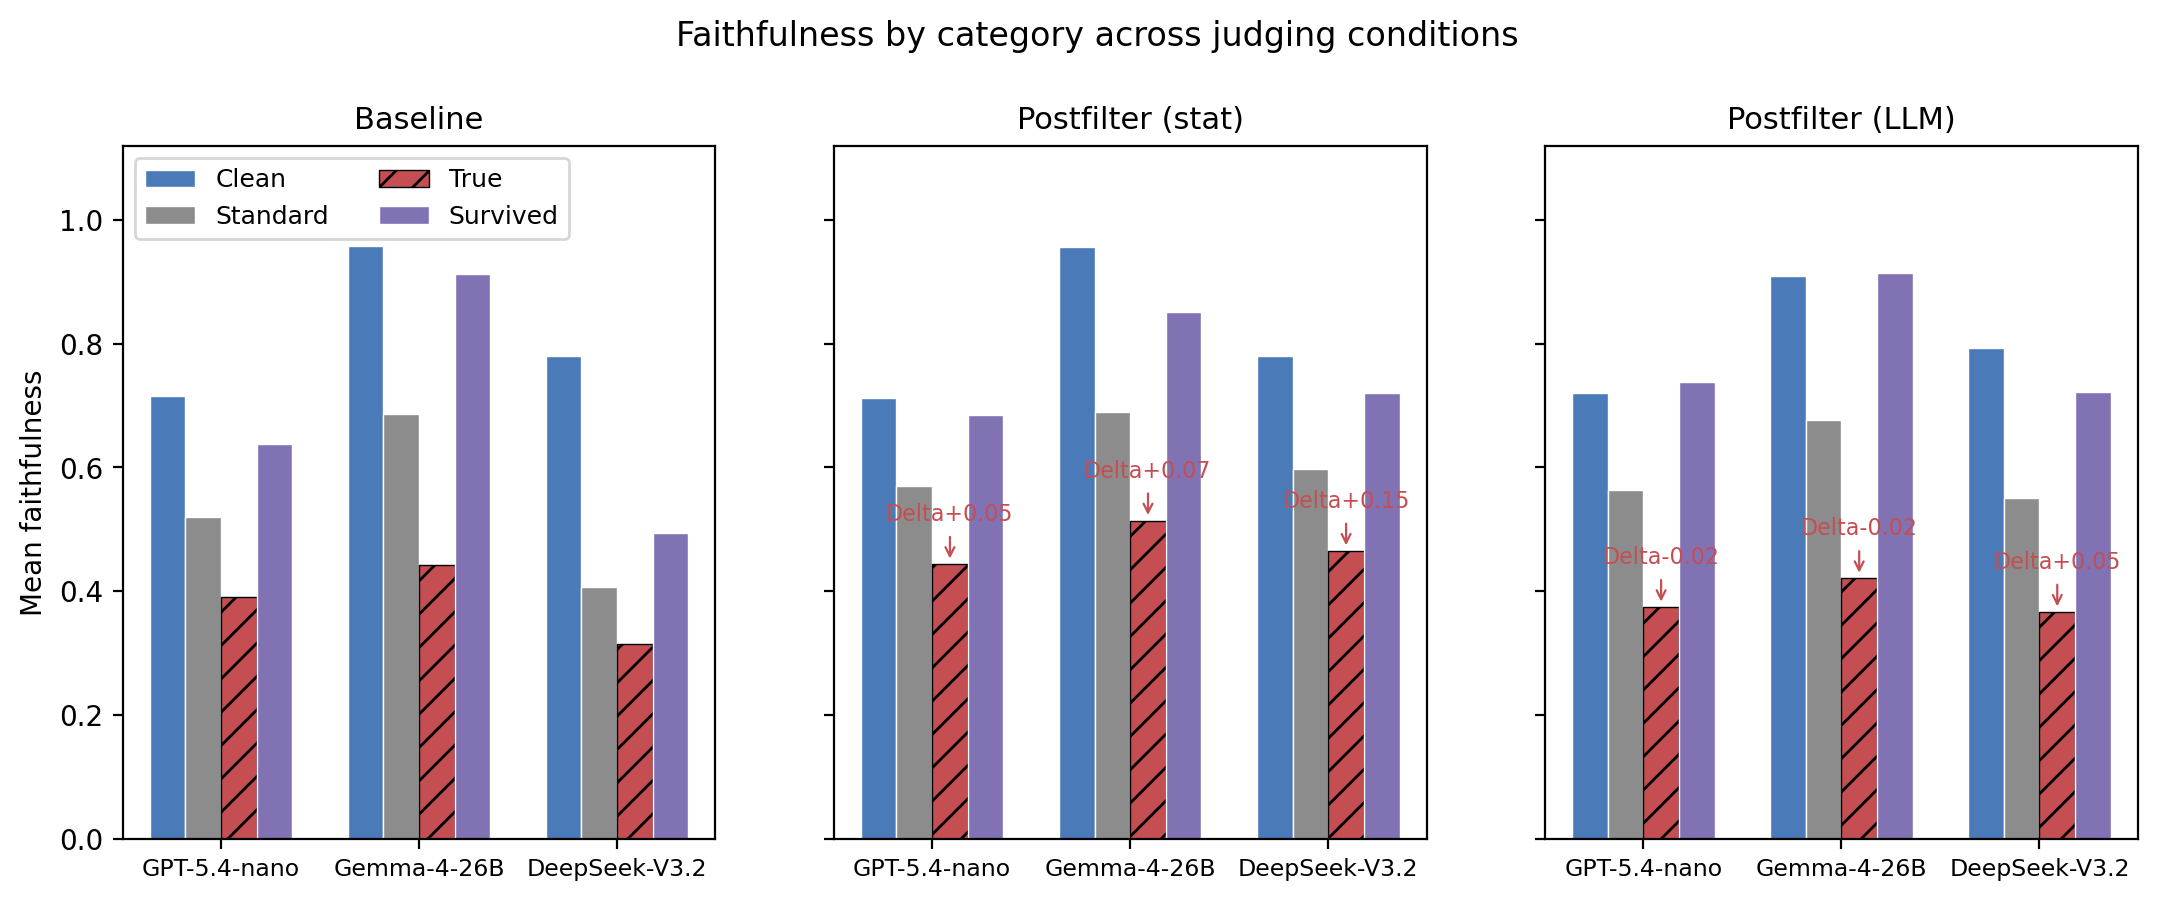
\includegraphics[width=0.95\textwidth]{../exports/figures/fig02_paradox_headline.png}
\caption{Mean faithfulness by category across baseline, statistical post-filtering, and LLM post-filtering. The True-category annotations show the change from baseline, where positive values indicate the filter-induced score increase.}
\label{fig:paradox-headline}
\end{figure}

The True column under postfilter is higher than the True column under baseline for all three judges. Filtering raises the rate at which judges score concentrated-poison contexts as faithful. The DeepSeek result is the most pronounced: baseline True mean of 0.314 jumps to 0.465 under the statistical filter - a 0.151 increase. GPT moves from 0.391 to 0.444, Gemma from 0.442 to 0.514. The statistical filter makes the worst case worse for every judge, with DeepSeek's effect roughly twice the magnitude of GPT's and Gemma's. The aggregate True-mean reported here averages over Type 1 (random noise) and Type 2 (adversarial fact rewriting) triplets, which contribute roughly equal counts but produce noticeably different per-injection effect sizes - for DeepSeek, +0.119 on random noise and +0.183 on adversarial fact, a 50\% relative difference. Section 4.4.4 reports the per-injection breakdown in detail.

The LLM filter (Mistral) shows a weaker and uneven pattern. DeepSeek's True mean rises by 0.053 under postfilter\_llm. GPT's drops by 0.017 and Gemma's drops by 0.022. The LLM filter does not modify content (Mistral classifies whole triplets rather than removing passages), so on True-category triplets - where the malicious passages have already overwritten supporting content - the filter has no opportunity to make the residual easier or harder for the judge. The DeepSeek effect is the only material True-mean change under the LLM filter.

The Survived column tells a more pronounced story. Survived means rise substantially under the statistical filter for GPT (0.638 → 0.685, Δ +0.047) and DeepSeek (0.494 → 0.720, Δ +0.226), and rise further under the LLM filter for both (GPT to 0.737, DeepSeek to 0.721). For Gemma the statistical filter reduces Survived by 0.061 (0.912 → 0.851), the only Survived cell where filtering visibly hurts. The Gemma decrease is consistent with its extreme-leniency calibration: Gemma's baseline Survived score is already near the ceiling, and the filter's collateral removal of supporting passages can only pull it down.

A compositional caveat: the Survived subset contains 112 random\_noise + 112 adversarial\_fact + 400 PoisonedRAG-style triplets, so PoisonedRAG-style is roughly 64\% of the Survived population. The aggregate Survived means in Table~\ref{tab:faithfulness-category-means} are therefore dominated by PoisonedRAG-style behaviour, not weighted across attack types in proportion to their adversarial sophistication. The DeepSeek Survived increase is largely the PoisonedRAG-style effect; the Type 1 and Type 2 contributions to Survived are smaller in magnitude and split in direction across judges. Section 4.4.4 examines the per-injection composition in detail and reports the magnitudes separately.

\begin{figure}[H]
\centering
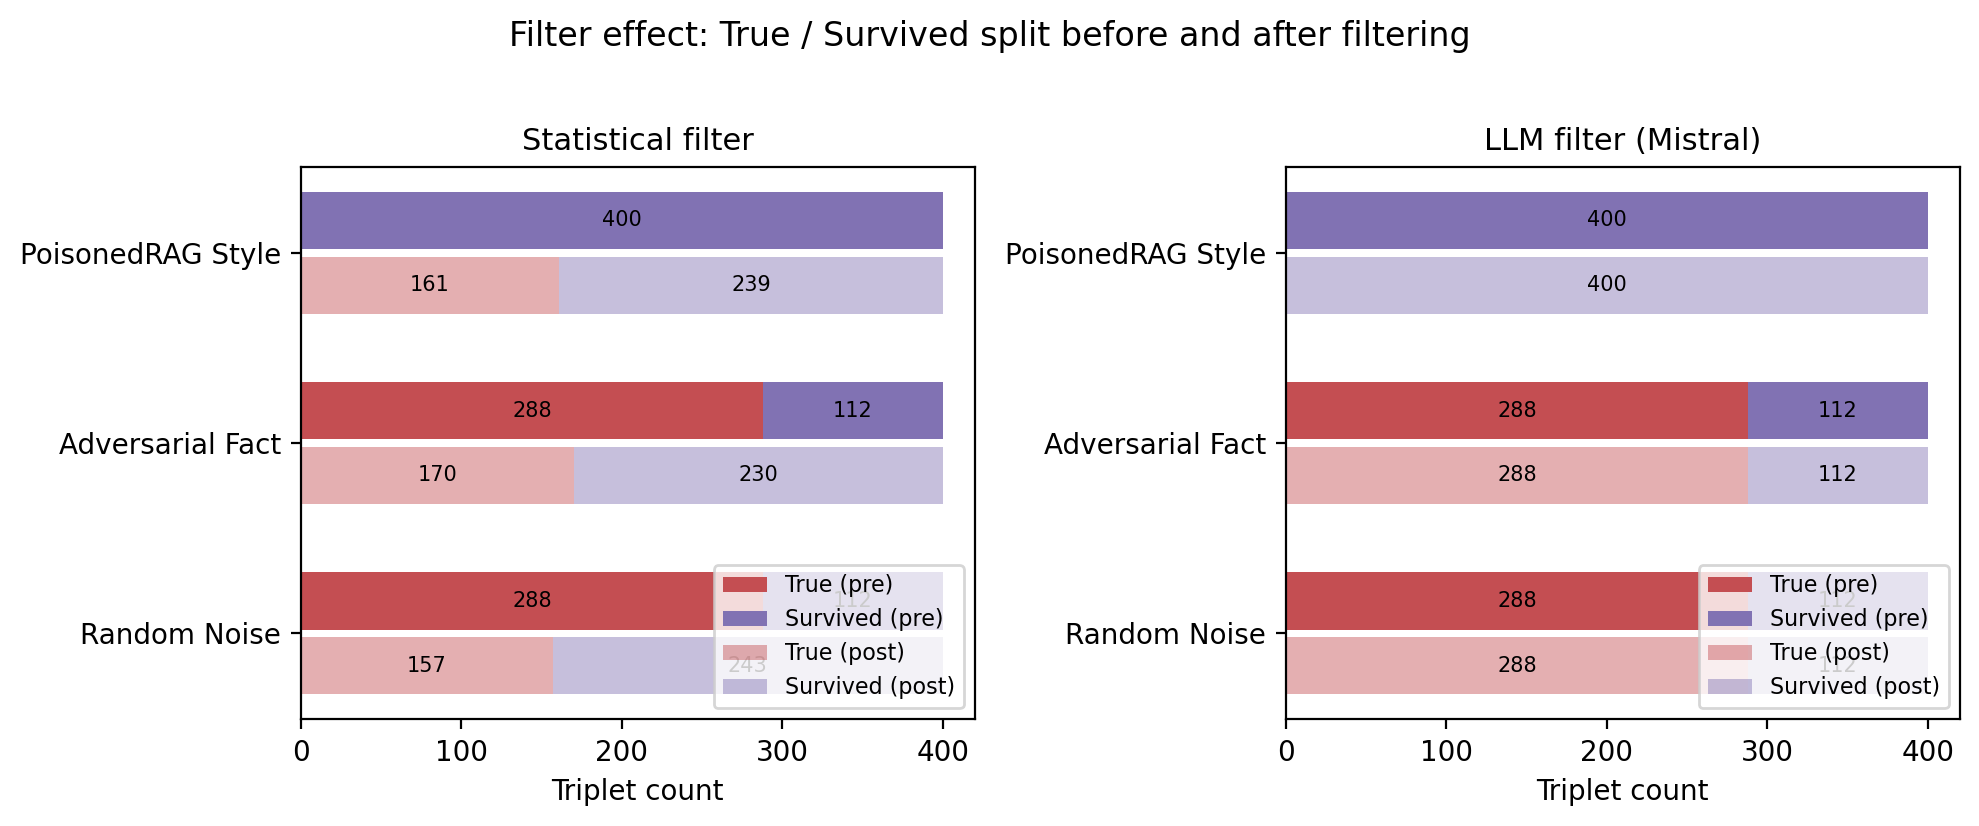
\includegraphics[width=0.95\textwidth]{../exports/figures/fig05_filter_behaviour.png}
\caption{Effect of the statistical and LLM filters on the True and Survived split of originally-poisoned triplets.}
\label{fig:filter-behaviour}
\end{figure}

\subsection{The picture across context relevance and answer relevance}

The faithfulness paradox in Table~\ref{tab:faithfulness-category-means} is partially specific to faithfulness. The other two RAGAS dimensions show the same direction in places but with different magnitudes and judge composition.

For context relevance, the True means under baseline are GPT 0.508, Gemma 0.695, DeepSeek 0.135. Under the statistical filter they are GPT 0.524, Gemma 0.666, DeepSeek 0.315. The DeepSeek context relevance shift (+0.180) is the largest True-subset paradoxical increase in the analysis. GPT's True context relevance is essentially unchanged (+0.016). Gemma's True context relevance actually decreases by 0.030 - one of two cells in the analysis where filtering visibly reduces a True-mean. The mechanism is the same as the faithfulness Survived decrease for Gemma: the baseline-True context relevance is already moderate-to-high (0.695), and the filter's collateral removal of supporting passages can only pull it down rather than make the residual look more relevant.

For answer relevance, all True-mean changes are small and uniformly positive (GPT +0.045, Gemma +0.031, DeepSeek +0.051). The shifts are smaller than for faithfulness or context relevance and consistent with the structural insensitivity of the metric noted in Section 4.1.1: answer relevance is largely about whether the answer is on-topic for the question, which is preserved regardless of context corruption. Answer relevance functions here as a methodological control showing that the True/Survived shifts on faithfulness and context relevance are not dominated by uniform changes in score-generation logistics across conditions.

The paradox's strength varies across metric: substantial on faithfulness and context relevance for DeepSeek, smaller but consistent on faithfulness for GPT and Gemma, and small on answer relevance throughout. The DeepSeek case is the cleanest example of the worst-case-worsened effect across two RAGAS dimensions; for the other judges, the pattern holds but more moderately. Detailed per-injection breakdowns are shown in Figures~\ref{fig:per-injection-faithfulness}--\ref{fig:per-injection-answer}.

\begin{figure}[H]
\centering
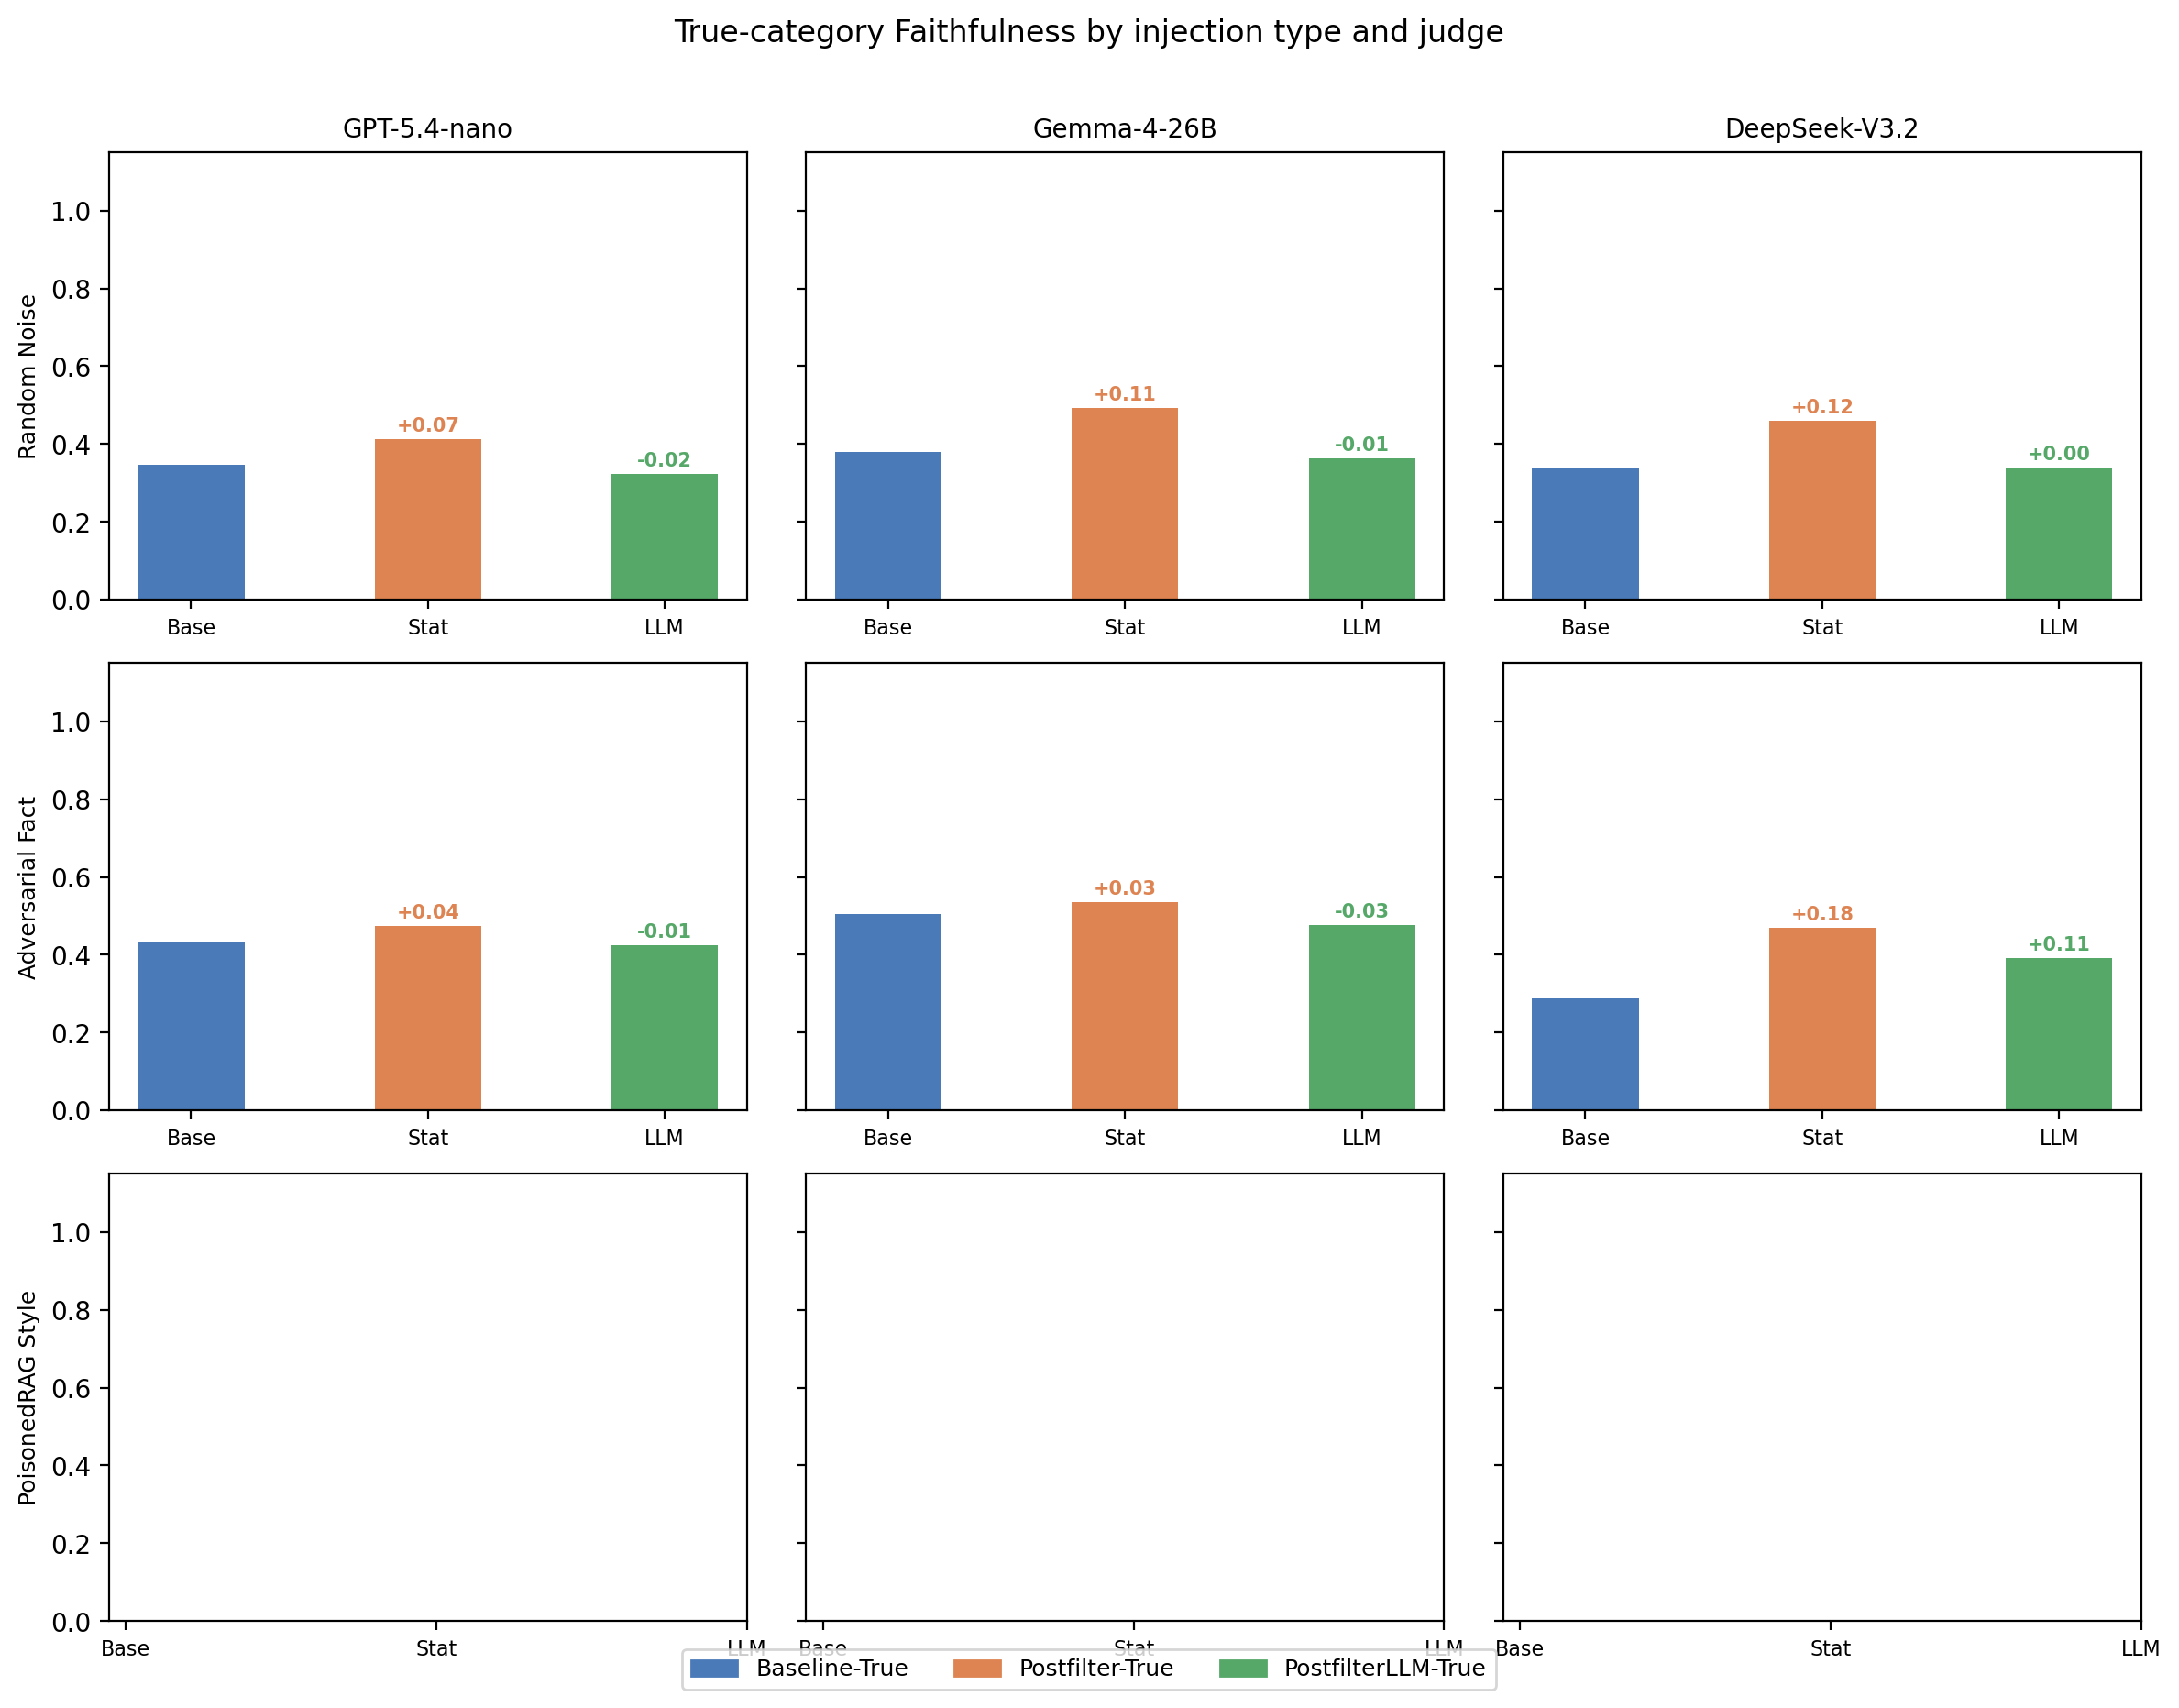
\includegraphics[width=0.95\textwidth]{../exports/figures/fig04a_per_injection_faithfulness.png}
\caption{True-category faithfulness by judge, injection type, and filtering condition.}
\label{fig:per-injection-faithfulness}
\end{figure}

\begin{figure}[H]
\centering
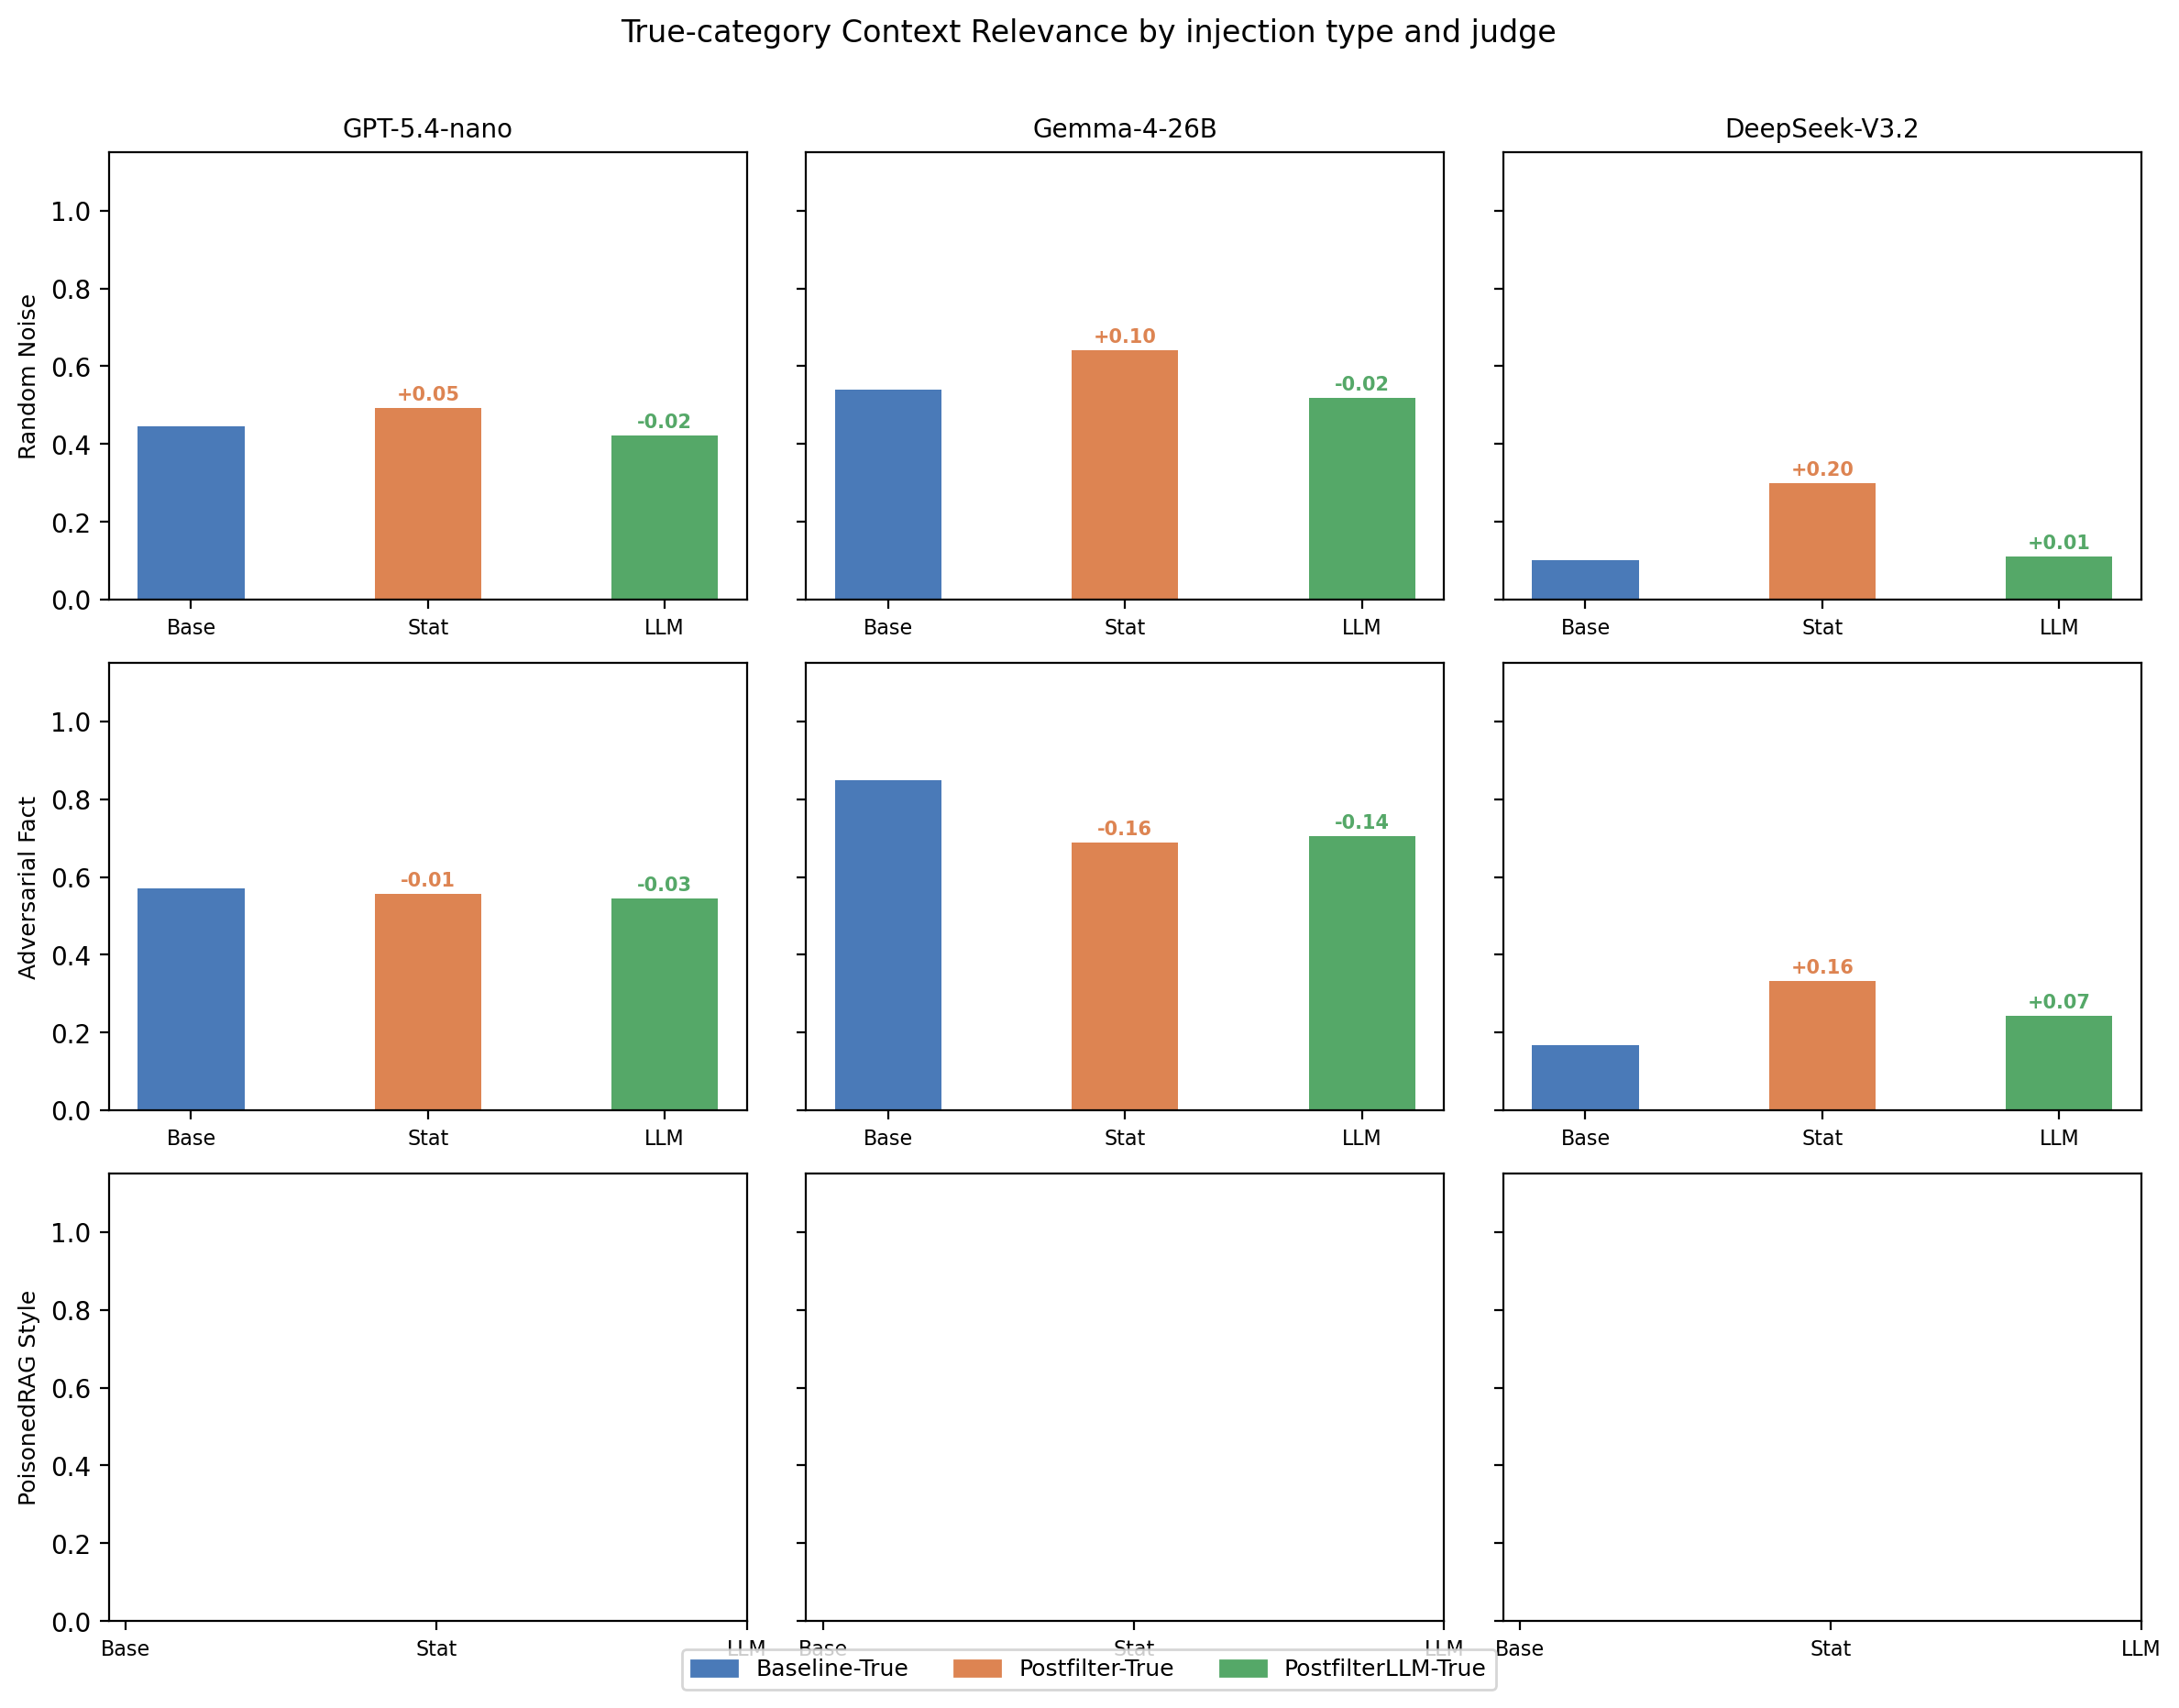
\includegraphics[width=0.95\textwidth]{../exports/figures/fig04b_per_injection_context.png}
\caption{True-category context relevance by judge, injection type, and filtering condition.}
\label{fig:per-injection-context}
\end{figure}

\begin{figure}[H]
\centering
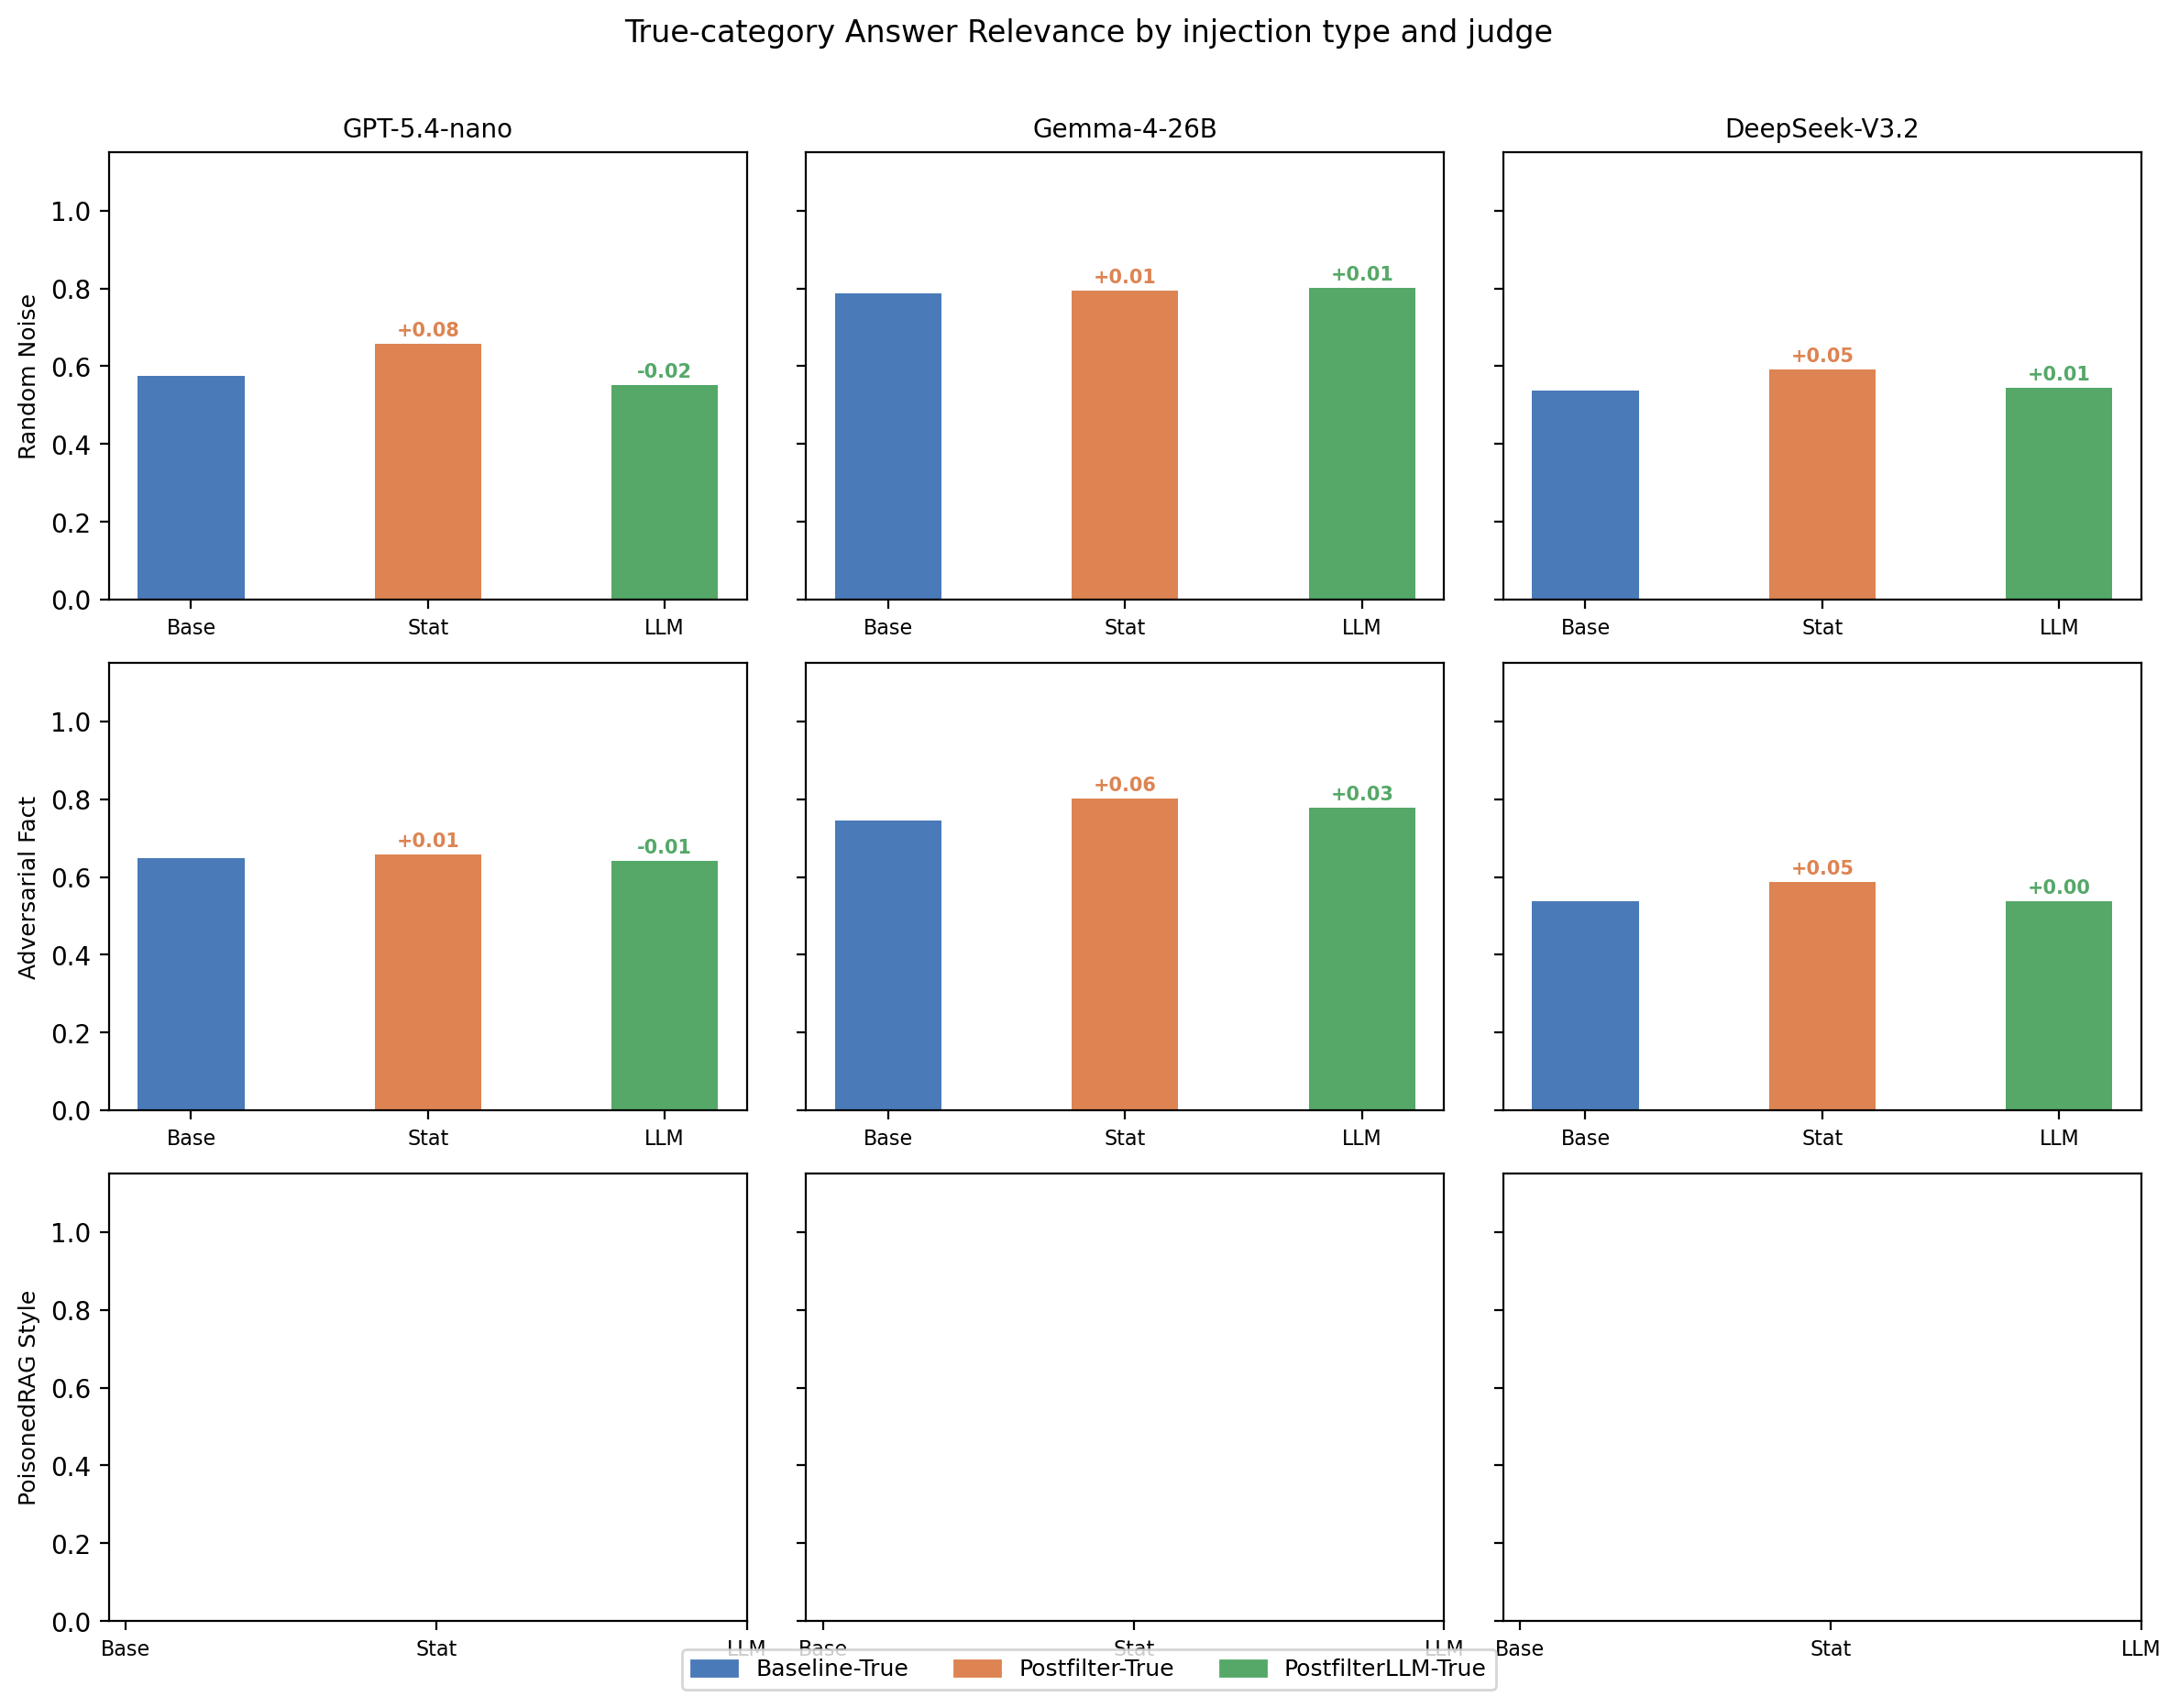
\includegraphics[width=0.95\textwidth]{../exports/figures/fig04c_per_injection_answer.png}
\caption{True-category answer relevance by judge, injection type, and filtering condition.}
\label{fig:per-injection-answer}
\end{figure}

\subsection{Per-injection magnitude}

The per-injection breakdown is structurally different across the True and Survived subsets, given that PoisonedRAG-style triplets all sit in Survived. We report the two subsets separately.

\textbf{True subset (random\_noise and adversarial\_fact only).} For DeepSeek under the statistical filter, baseline-True faithfulness vs postfilter-True faithfulness:

\begin{itemize}
  \item Random noise: 0.340 → 0.460 (Δ +0.119)
  \item Adversarial fact: 0.287 → 0.470 (Δ +0.183)
\end{itemize}

For GPT the same comparison: random noise 0.347 → 0.413 (Δ +0.065), adversarial fact 0.434 → 0.474 (Δ +0.040). For Gemma: random noise 0.379 → 0.493 (Δ +0.114), adversarial fact 0.506 → 0.535 (Δ +0.030). The True-subset paradox is moderate-to-large for DeepSeek, moderate for Gemma on random noise, and small for the others. Adversarial fact and random noise behave similarly within each judge, with no strong injection-type-specific pattern in the True subset.

\textbf{Survived subset (all three injection types, with PoisonedRAG-style dominating numerically).} Survived means under the statistical filter shift dramatically for PoisonedRAG-style triplets, where the residual after filtering is the most consequential. For DeepSeek on PoisonedRAG-style: baseline Survived 0.361 → postfilter 0.738 (Δ +0.377). This is the single largest cell-level effect in the analysis. For GPT on PoisonedRAG-style: 0.570 → 0.709 (Δ +0.139). For Gemma on PoisonedRAG-style: 0.885 → 0.914 (Δ +0.029, ceiling effect).

The Survived effects on adversarial\_fact and random\_noise are smaller and split in direction: GPT and Gemma Survived means on those types decrease modestly (consistent with collateral support loss), while DeepSeek Survived means rise modestly. The PoisonedRAG-style Survived effect dominates the aggregate because (i) Type 3 contributes 400 of the 624 Survived triplets per cell and (ii) its post-filter mean shifts farther than any other injection type's. Per-injection patterns for all judges and conditions are shown in Figure~\ref{fig:per-injection-faithfulness}.

The likely mechanism behind the PoisonedRAG-style Survived shift is consistent with the broader picture developed in Section 4.5.2: filtering produces a shorter, more topically focused residual through the removal of original distractor passages, and judges score the cleaner-looking residual as more faithful regardless of whether the surviving content actually supports the answer. PoisonedRAG-style triplets are particularly susceptible because they contain highly polished malicious passages alongside intact supporting context. At baseline, the judge sees a mixture: original supporting passages plus polished poison plus original distractors, and DeepSeek's near-binary scoring (Section 4.1.3) registers the contradiction reliably. After the statistical filter runs, it removes the more conspicuous distractors and some of the malicious passages, leaving the most polished malicious content alongside the supporting passages in a context that is shorter, less noisy, and more credible-looking. The judge revises its faithfulness verdict upward. The DeepSeek PoisonedRAG-style postfilter Survived mean of 0.738 is what this looks like in the cell.

We treat this mechanism story as a plausible interpretation rather than a proven causal claim. The strongest evidence comes from the distractor-removal stratification (Section 4.5.2), which shows the True-subset Δ rising monotonically with the number of distractors removed, plus the post-filter length correlation (r ≈ 0.31–0.47 across judges) which is much stronger than at baseline. The earlier hypothesis that the paradox is driven by collateral removal of supporting passages is empirically refuted in Section 4.5.2; collateral damage happens but moves scores in the opposite direction.

\subsection{Statistical significance}

McNemar's paired test on triplet-level FPR-threshold-crossings detects the True-category shifts at conventional levels when triplets are treated as independent observations: GPT χ² = 8.16 (p = 0.004), Gemma χ² = 10.93 (p < 1e-3), DeepSeek χ² = 34.40 (p < 1e-8) on the True subset under the statistical filter. This treatment is, however, optimistic: the 1,200 poisoned triplets derive from 100 base questions, with each question contributing twelve triplets (three injection types × four noise levels). Triplets sharing a base question share the question text, the ground-truth answer, and the original supporting passages, and are therefore not independent observations.

A question-clustered bootstrap (1,000 iterations resampling at the base-question level) gives the more honest picture. The 95\% bootstrap confidence intervals for the True-subset χ² values are wide and span low values for two of the three judges:

\begin{table}[H]
\centering
\small
\resizebox{\textwidth}{!}{%
\begin{tabular}{lllll}
\toprule
Judge & Condition & Uncorrected χ² & Bootstrap 95\% CI & Bootstrap-corrected p \\
\midrule
GPT & postfilter & 8.16 & [0.12, 16.34] & 0.239 \\
Gemma & postfilter & 10.93 & [0.11, 21.82] & 0.259 \\
DeepSeek & postfilter & 34.40 & [7.26, 41.83] & 0.099 \\
DeepSeek & postfilter\_llm & 15.57 & [2.70, 18.27] & 0.089 \\
\bottomrule
\end{tabular}
}
\caption{McNemar paired test on True-subset faithfulness threshold-crossings (≥0.5). Uncorrected χ² and p-values treat triplets as independent. Bootstrap-corrected values resample at the base-question level (n=100 questions, 1,000 iterations), accounting for within-question correlation across noise levels and injection types.}
\label{tab:mcnemar-true-faithfulness}
\end{table}

\begin{figure}[H]
\centering
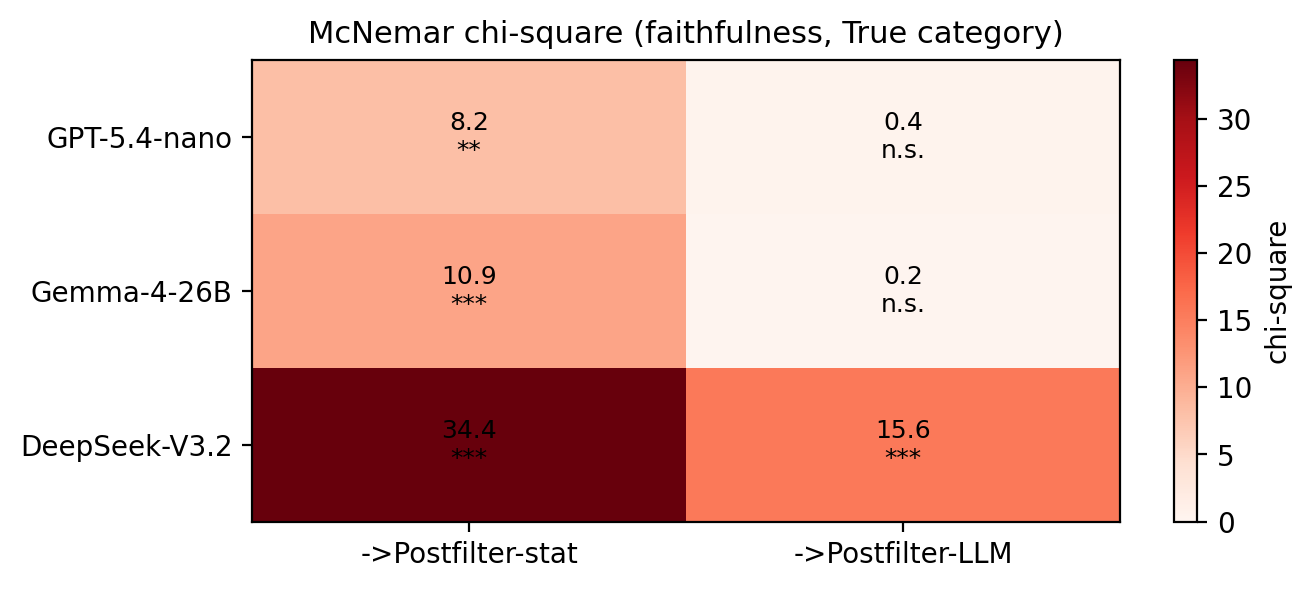
\includegraphics[width=0.80\textwidth]{../exports/figures/fig07_mcnemar.png}
\caption{McNemar test statistic for faithfulness threshold-crossing changes in the True category, comparing baseline with each post-filter condition.}
\label{fig:mcnemar}
\end{figure}

After clustered correction, GPT and Gemma's True-subset shifts under the statistical filter are no longer significant at conventional thresholds; their bootstrap CIs include zero. DeepSeek's True-subset effect is borderline (p = 0.099). The Survived-subset effects tell a different story - the DeepSeek Survived shift, which traces almost entirely to PoisonedRAG-style triplets, remains robustly significant under clustered bootstrap (χ² = 77.7, bootstrap CI [29.6, 73.4], corrected p = 0.012 under the statistical filter; corrected p < 0.001 under the LLM filter). The largest single end-to-end effect in the analysis is also the most statistically robust.

The implication is that the True-subset paradox is directional and visible across all three judges but is not, with the data we have, decisively significant for GPT or Gemma once question-level clustering is accounted for. The Survived-subset effect on PoisonedRAG-style triplets is robust under any reasonable correction. The thesis's central claim - that filtering reshapes judge response in counterintuitive ways - is best supported by the Survived-subset result on the most adversarial attack class, not by the True-subset shifts on Types 1 and 2 alone.

\subsection{The reverse across noise levels}

The end-to-end behaviour reverses partially across noise levels - and in a direction that is operationally important. At low noise levels (0.2, where only 20\% of context was replaced), the True mean under the statistical filter is highest. At high noise levels (0.8, where 80\% of context was replaced), the True mean is lower, even if still above baseline-True.

For DeepSeek under the statistical filter, postfilter-True faithfulness by noise level: 0.671 at noise=0.2, 0.652 at noise=0.4, 0.468 at noise=0.6, falling to 0.244 at noise=0.8. The pattern reverses the baseline from Section 4.1.4, where higher noise was easier for the judge. After filtering, lower noise is the harder case, with the postfilter-True mean dropping by more than 0.4 across the noise range.

The mechanism is straightforward in retrospect. At noise=0.2, only one or two passages were replaced. The filter removes the most obvious among those. The residual is mostly clean passages plus the supporting passages - a context that reads as well-formed, polished, and topically coherent. The judge reads this context, sees no obvious anomaly, and scores the answer as faithful. At noise=0.8, the filter is removing many more passages. The residual is sparse and visibly degraded. The judge correctly reads this as untrustworthy and scores low.

The implication for deployment is uncomfortable. Subtle, low-noise attacks are exactly the threats that an upstream filter should be best positioned to handle, because the filter has more clean context to work with. Instead, low-noise attacks become more dangerous post-filter than they were at baseline, because the filter's success at removing the poison produces a residual that looks more trustworthy than it is.

\begin{figure}[H]
\centering
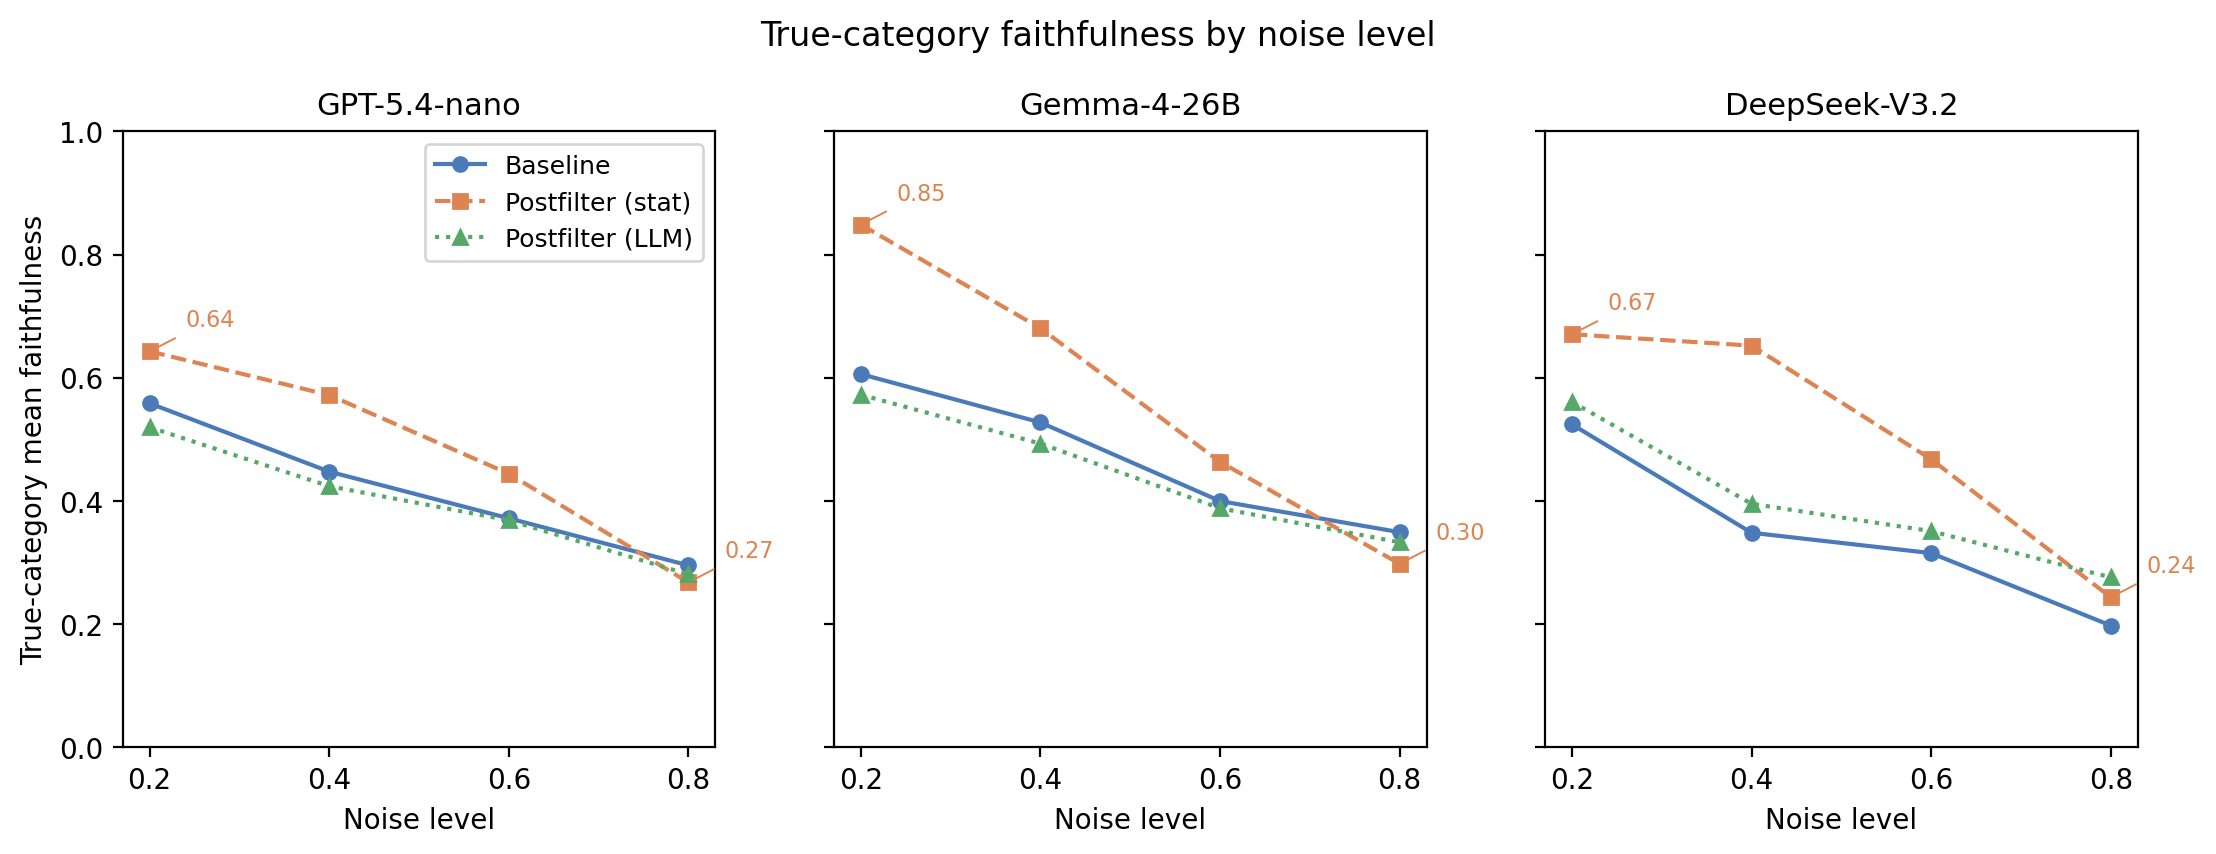
\includegraphics[width=0.95\textwidth]{../exports/figures/fig03_true_mean_by_noise.png}
\caption{True-category mean faithfulness by noise level under baseline, statistical post-filtering, and LLM post-filtering.}
\label{fig:true-mean-noise}
\end{figure}

\section{Filter Behaviour Audit}

The end-to-end results in Section 4.4 raise a mechanism question. Why does the filter, which is a strong classifier (F1 = 0.929 on the test set), make judge behaviour worse on the True subset? Section 4.5 audits what the filter actually did at the passage level and surfaces a finding that explains part of the answer.

\subsection{What the statistical filter removed}

For each originally-poisoned triplet, we record three counts after the statistical filter runs: how many poisoned passages were correctly removed, how many were missed, and how many \textit{originally-supporting} passages were removed (collateral damage).

Table~\ref{tab:filter-audit-by-injection} summarises by injection type.

\begin{table}[H]
\centering
\small
\resizebox{\textwidth}{!}{%
\begin{tabular}{llllll}
\toprule
Injection type & Mean poisoned per triplet & Mean caught & Mean missed & Mean supporting lost (collateral) & Recall \\
\midrule
Random noise & 4.98 & 2.76 & 2.22 & 0.32 & 0.554 \\
Adversarial fact & 4.98 & 2.74 & 2.23 & 0.33 & 0.551 \\
PoisonedRAG-style & 4.98 & 1.48 & 3.50 & 0.39 & 0.296 \\
\bottomrule
\end{tabular}
}
\caption{Statistical filter passage-level behaviour by injection type. The "supporting lost" column counts originally-supporting passages that were wrongly flagged and removed by the filter.}
\label{tab:filter-audit-by-injection}
\end{table}

\begin{figure}[H]
\centering
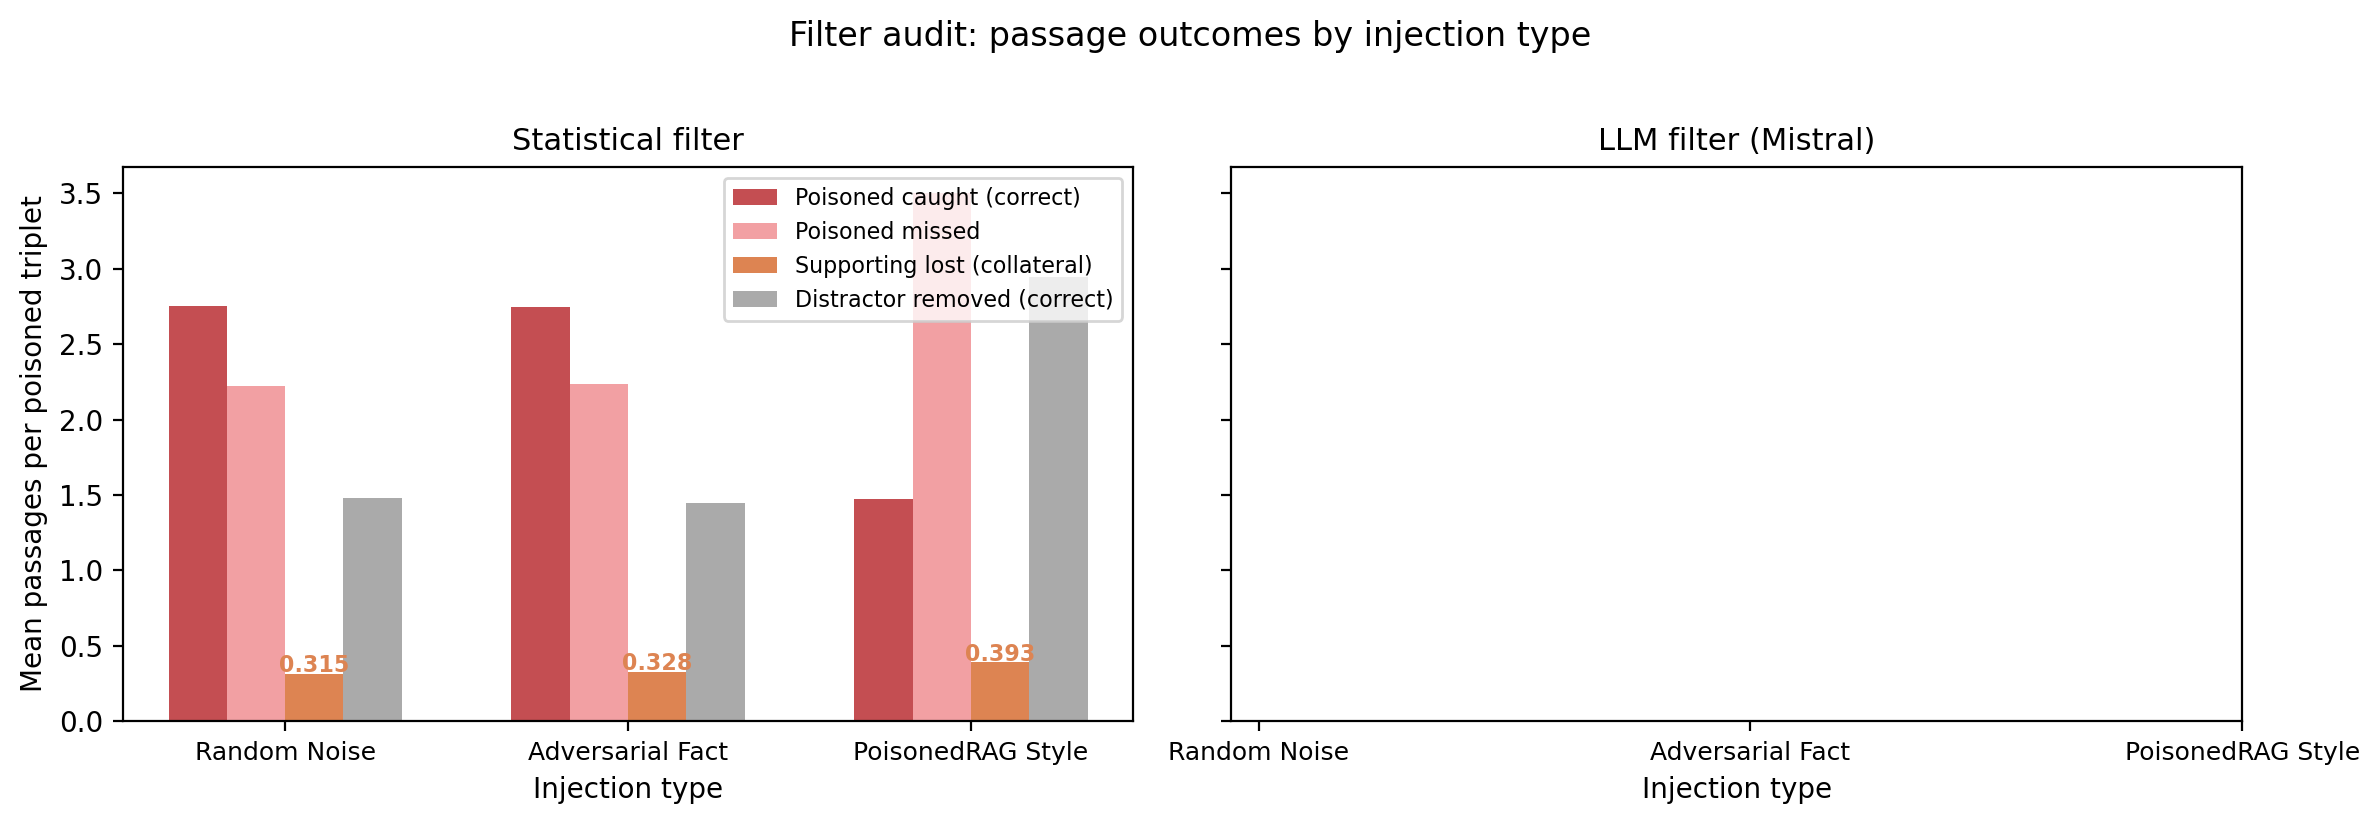
\includegraphics[width=0.95\textwidth]{../exports/figures/fig08_filter_audit.png}
\caption{Passage-level filter audit by injection type, including correctly caught poison, missed poison, and collateral removal of supporting passages.}
\label{fig:filter-audit}
\end{figure}

Two observations from this table.

First, the per-triplet recall (mean caught divided by mean poisoned) is substantially below the test-set recall reported in Section 4.2. The test-set numbers are computed on a held-out evaluation split where the classifier operates at its trained operating point. The whole-dataset audit, which includes triplets the classifier saw during training and validation, shows a more conservative effective recall - the headline 0.929 F1 reflects classifier performance, not the rate at which poison is fully eliminated from a random triplet.

Second, and more importantly, the filter removes about 0.32 to 0.39 originally-supporting passages per triplet (averaging across the full Poisoned Evaluation Dataset). Each triplet has only two supporting passages by HotpotQA construction, so a loss of 0.35 corresponds to roughly 17.5\% of supporting passages being removed as collateral damage. This is not a small effect.

A test-split-only re-audit shows that the collateral-loss figure varies modestly with the data partition. On the test split alone (n=80 originally-poisoned triplets per injection type), the mean supporting-passages-lost figures are 0.21 (random\_noise), 0.43 (adversarial\_fact), and 0.38 (poisonedrag\_style). The full-dataset and test-only numbers differ by 0.05 or more for adversarial\_fact and random\_noise, reflecting the fact that the DeBERTa classifier has seen the training-set passages during fitting and behaves slightly differently on unseen data. The full-dataset 0.345 figure should therefore be read as an in-sample aggregate; the deployment-relevant collateral-loss rate is the test-only value, and it depends on the injection type.

\subsection{What is actually driving the True-subset shift}

A naive reading of the filter audit suggests the collateral damage matters: the filter removes supporting passages 17.5\% of the time, depriving the judge of evidence it would otherwise use to detect a contradiction. We tested this directly. The counterfactual is straightforward: if collateral damage is the operative mechanism, then within the True subset, triplets where the filter removed at least one supporting passage should show the largest paradoxical Δ (judge gains the most when it has the least supporting evidence). Triplets where the filter removed zero supporting passages should show a smaller Δ.

Table~\ref{tab:support-removal-stratified} reports the result.

\begin{table}[H]
\centering
\small
\resizebox{\textwidth}{!}{%
\begin{tabular}{llllll}
\toprule
Judge & Support removed by filter & n triplets & Baseline True mean & Postfilter True mean & Δ \\
\midrule
GPT & Yes (≥1) & 157 & 0.443 & 0.282 & \textbf{−0.161} \\
GPT & No (0) & 419 & 0.371 & 0.504 & +0.133 \\
Gemma & Yes (≥1) & 157 & 0.532 & 0.305 & \textbf{−0.227} \\
Gemma & No (0) & 419 & 0.409 & 0.592 & +0.184 \\
DeepSeek & Yes (≥1) & 157 & 0.452 & 0.305 & \textbf{−0.147} \\
DeepSeek & No (0) & 419 & 0.262 & 0.525 & +0.263 \\
\bottomrule
\end{tabular}
}
\caption{True-subset Δ stratified by whether the statistical filter removed at least one supporting passage. The paradox (Δ > 0) appears only in triplets where supporting passages survived the filter. In triplets where collateral damage occurred, scores drop substantially in all three judges.}
\label{tab:support-removal-stratified}
\end{table}

The result is the opposite of what the collateral-damage hypothesis predicts. In all three judges, when the filter removed supporting context, faithfulness scores fell by 0.15 to 0.23 - the judge correctly detected the resulting evidential gap. The paradox (post-filter scores rising) emerges entirely in triplets where the filter spared the supporting passages. Collateral damage is a real phenomenon (it happens 17.5\% of the time and produces the expected score drops) but it is not the operative cause of the True-subset paradox.

Two alternative mechanisms are consistent with the corrected picture: context shortening through distractor removal, and a length-driven shift in judge calibration. We tested both.

\textbf{Distractor removal.} For each True-subset triplet under the statistical filter, we computed the number of original HotpotQA distractor passages the filter removed correctly. Table~\ref{tab:distractor-removal-stratified} stratifies the True-mean Δ by the quartile of distractor removal.

\begin{table}[H]
\centering
\small
\resizebox{\textwidth}{!}{%
\begin{tabular}{llllll}
\toprule
Judge & Distractor removal quartile & n & Baseline True mean & Postfilter True mean & Δ \\
\midrule
GPT & Q1 (low) & 291 & 0.410 & 0.347 & −0.063 \\
GPT & Q2 & 210 & 0.368 & 0.510 & +0.142 \\
GPT & Q3 (high) & 75 & 0.383 & 0.633 & \textbf{+0.251} \\
Gemma & Q1 (low) & 291 & 0.467 & 0.379 & −0.088 \\
Gemma & Q2 & 210 & 0.399 & 0.597 & +0.198 \\
Gemma & Q3 (high) & 75 & 0.468 & 0.803 & \textbf{+0.335} \\
DeepSeek & Q1 (low) & 291 & 0.340 & 0.335 & −0.005 \\
DeepSeek & Q2 & 210 & 0.290 & 0.547 & +0.257 \\
DeepSeek & Q3 (high) & 75 & 0.280 & 0.741 & \textbf{+0.461} \\
\bottomrule
\end{tabular}
}
\caption{True-subset Δ stratified by quartile of original distractor passages removed by the statistical filter. The paradox grows monotonically with the number of distractors removed, in all three judges. The largest Δ in the high-quartile cell (Q3) reaches +0.461 for DeepSeek and +0.335 for Gemma.}
\label{tab:distractor-removal-stratified}
\end{table}

The pattern is monotonic in all three judges. Triplets where the filter removed few distractors show no paradox (or a small negative Δ). Triplets where the filter removed many distractors show a large paradox (Δ +0.25 to +0.46). The mechanism is not collateral damage; it is context clarification through distractor removal. The original HotpotQA distractor passages, which the dataset constructors included precisely to make the multi-hop task harder, are noisy and topically loose. The statistical filter, designed to remove poisoned passages, also removes many of these original distractors. The residual is shorter and more topically focused - and judges score this cleaner residual as more faithful, regardless of whether it actually contains the supporting evidence needed to answer the question correctly.

\textbf{Length effect.} The mechanism above predicts that post-filter contexts should be shorter on average and that judge scores should correlate with context length more strongly post-filter than at baseline. Both predictions hold. Mean post-filter context length is 7.11 passages versus 11.62 at baseline, a 39\% reduction. The Pearson correlation between context length and faithfulness score is weak at baseline (r = 0.099 GPT, 0.290 Gemma, −0.082 DeepSeek) and substantially stronger post-filter (r = 0.357 GPT, 0.468 Gemma, 0.312 DeepSeek). After filtering, judges score shorter contexts as more faithful.

These results require us to revise the mechanism story given in Section 4.4. The end-to-end paradox is not driven by the polished-poison residual or by collateral damage in any direct sense. It is driven by the filter's incidental removal of original HotpotQA distractors, which produces a shorter and more topically focused residual that the judge reads as cleaner, more coherent, and therefore more faithful. The remaining poison sits inside this cleaner-looking residual and benefits from its credibility. The collateral-damage phenomenon happens but moves scores in the opposite direction: when the filter does kill supporting passages, the judge correctly detects the evidential gap and scores lower. The aggregate True-subset paradox we report in Section 4.4 is the net of these two mostly-opposing effects, with the distractor-removal effect dominating numerically.

\subsection{LLM filter audit}

The LLM filter (Mistral) does not modify passages, so the collateral-damage analysis does not apply in the same form. Mistral classifies each triplet as poisoned or not, and in deployment a flagged triplet would be excluded entirely. The audit-relevant quantity for Mistral is the per-attack triplet-level recall and false-alarm rate, already reported in Table~\ref{tab:mistral-filter-by-injection}: recall ranges from 0.140 (random noise) to 0.765 (PoisonedRAG-style), and clean-FPR is around 0.17 across all attack types.

The LLM filter does not exhibit the collateral-damage mechanism by construction. It exhibits a different limitation: low recall on subtle attacks, particularly random noise. Of the two filters, the statistical filter catches more poison but at the cost of removing some legitimate supporting context; the LLM filter is more conservative about modifying triplets but lets more poison through. Neither cleanly avoids the underlying problem of producing residuals (or routing decisions) that improve judge reliability end-to-end.

\section{Justification Analysis}

The justification analysis re-scores a 28-triplet subset under three prompt conditions: a standard scoring prompt (the same prompt used in the main experiments), a standard prompt applied after the statistical pre-filter has run, and a poison-aware prompt that explicitly describes the three attack types before asking for scores. The subset is stratified across the three injection types and is scored only by GPT-5.4-nano (the judge with continuous calibration, where score variation is most informative).

The poison-aware prompt produces a substantial shift on the two engineered attack types. For PoisonedRAG-style triplets, mean faithfulness drops from 0.800 under the standard prompt to 0.492 under the poison-aware prompt (Δ −0.308). For adversarial-fact triplets, the same prompt produces a drop from 0.758 to 0.558 (Δ −0.200). For random-noise triplets, the change is smaller in magnitude but still in the same direction (0.600 to 0.517, Δ −0.083). The standard-postfilter condition shows a different pattern: faithfulness on PoisonedRAG-style stays high (0.830, essentially unchanged from the standard 0.800), faithfulness on adversarial fact drops modestly (0.666), and faithfulness on random noise collapses to 0.233. This split is consistent with the distractor-removal mechanism in Section 4.5.2: the statistical filter removes the noisy random-noise injections aggressively, exposing the residual as visibly degraded, while the polished PoisonedRAG-style content survives the filter and inherits the credibility of a cleaner-looking residual.

Two qualitative observations from the reasoning text reinforce the score patterns. First, on PoisonedRAG-style triplets where the poison-aware prompt elicits low faithfulness scores, the judge's justification text identifies the adversarial passage explicitly - naming the contradiction with the ground-truth answer or flagging the retrieval-optimised structure. The judge can identify the attack when primed to look for it. Second, on adversarial-fact triplets, the justification text often correctly flags the contradiction in the reasoning even when the numerical score remains relatively high. The judge's reasoning recognises the attack but its scoring does not always reflect the recognition.

The sample size (28 triplets, single judge, three prompt conditions) is too small to support strong statistical claims. We report the analysis as a qualitative supplement to the main results: it suggests that explicit prompting can mitigate the engineered attack types more than it does random noise, that filter-then-judge interacts non-trivially with attack type (helpful on random noise, neutral or worse on PoisonedRAG-style), and that the gap between judge reasoning and judge scoring is itself a phenomenon worth further study. The full prompt texts and a representative sample of justifications are included in Appendix B.

\section{Multi-Judge Disagreement}

We compute, for each triplet at baseline, the standard deviation of faithfulness scores across the three judges (GPT, Gemma, DeepSeek) and correlate the per-triplet std with the binary \texttt{is\_poisoned} ground-truth label.

The Pearson correlation is r = +0.113 (p < 1e-6, n = 2,397 triplets where all three judges produced scores). The mean inter-judge std on poisoned triplets is 0.256; on clean triplets it is 0.205. Poisoned triplets produce slightly more disagreement than clean ones, and the difference is statistically significant given the sample size, but the effect is small in magnitude. (We note separately that the cross-judge correlation between GPT and DeepSeek faithfulness scores is r = +0.514. This is a different quantity - it asks whether the two judges tend to score the same triplet similarly - and confirms only that the judges are not independent samples of the underlying judgement task.)

The practical implication is that ensemble-based detection (flagging triplets where the three judges disagree most) is not viable as a poisoning detector. A correlation of 0.113 explains roughly 1\% of the variance in the poisoning label, far too little to support a thresholded decision. We confirmed this directly: a mean-score ensemble (averaging the three judges' faithfulness scores and thresholding at 0.5) produces a faithfulness FPR of 0.555 - worse than DeepSeek's individual baseline of 0.412. A majority-vote ensemble produces 0.575. Neither ensemble improves over the best individual judge.

A secondary finding worth noting: when we restrict to poisoned triplets only and correlate per-triplet inter-judge std with injection-type ordinal severity (random noise = 0, adversarial fact = 1, PoisonedRAG-style = 2), the correlation is r = +0.287. Inter-judge disagreement grows with attack sophistication. Judges agree on what random noise looks like and disagree on what PoisonedRAG-style looks like. This is consistent with the cross-judge calibration divergence on PoisonedRAG-style reported in Section 4.1.3.

This is a useful negative result. It rules out a tempting but ineffective mitigation. Practitioners considering ensemble methods for adversarial-RAG defence should not expect them to recover detection sensitivity that the constituent judges lack individually. The disagreement signal exists but is too weak to operationalise.

\begin{figure}[H]
\centering
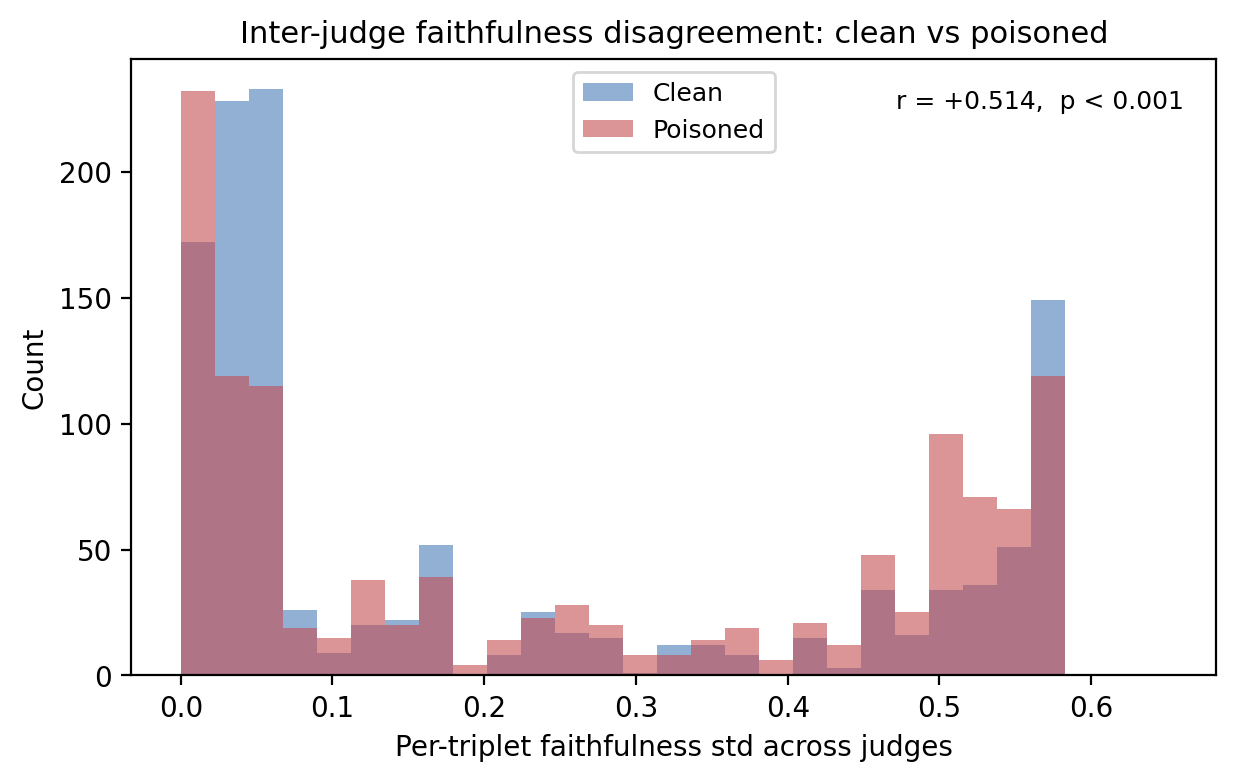
\includegraphics[width=0.80\textwidth]{../exports/figures/fig06_inter_judge_variance.png}
\caption{Distribution of per-triplet faithfulness disagreement across judges, separated by clean and poisoned triplets.}
\label{fig:interjudge-variance}
\end{figure}

\section{Summary of Findings}

The empirical findings of Chapter 4 can be summarised in seven points.

First, the three judges fail at substantial rates on baseline poisoned context. Faithfulness FPRs range from 0.412 (DeepSeek) to 0.555 (GPT) to 0.699 (Gemma). LLM-as-a-Judge under corpus poisoning is a real vulnerability with magnitude that is operationally significant.

Second, the three judges occupy distinct calibration regimes (continuous, near-binary, extreme-leniency) and respond differently to attack class. GPT and Gemma find PoisonedRAG-style attacks hardest; DeepSeek finds them easiest. Within our panel, scoring strategy appears to matter at least as much as judge size or training compute for robustness; whether this generalises beyond three judges is an open question.

Third, the multi-signal statistical pre-filter performs well as a classifier on the held-out test set (F1 = 0.929, precision = 0.955, recall = 0.904, clean FPR = 0.012). The filter's strongest recall is on PoisonedRAG-style (1.000), driven by the embedding cosine signal exploiting the retrieval-optimisation property of these attacks.

Fourth, the LLM-based pre-filter (Mistral, triplet-level) performs less well as a classifier (F1 = 0.601) and shows a sharp asymmetry by attack type - strong on PoisonedRAG-style (recall 0.765), weak on random noise (recall 0.140). The two filters detect partially complementary phenomena.

Fifth, end-to-end the picture is paradoxical. Decomposing originally-poisoned triplets into True (supporting passages overwritten) and Survived (supporting passages intact), filtering raises True-category faithfulness for all three judges under the statistical filter (Δ +0.053 GPT, +0.072 Gemma, +0.151 DeepSeek). Under the LLM filter the True-subset effect is significant only for DeepSeek (+0.053). On context relevance the paradox is concentrated on DeepSeek (+0.180). The largest single end-to-end effect is in the Survived subset for PoisonedRAG-style: DeepSeek's Survived faithfulness rises by 0.377 under the statistical filter, driven by the polished residual that emerges when the filter removes the noisier malicious passages and leaves the most fluent ones alongside intact supporting context. Filtering makes the worst case (True) worse for all judges, and in DeepSeek's case dramatically transforms the easier case (Survived) when faced with PoisonedRAG-style attacks.

Sixth, the operative mechanism behind the True-subset shifts is not what we initially conjectured. We tested two candidate mechanisms empirically. The collateral-damage mechanism - filter removes supporting passages and the judge loses contradicting evidence - is refuted by the data: in triplets where the filter removed a supporting passage, scores fell by 0.15–0.23 across all three judges. The paradox emerges only in triplets where the filter spared the supporting passages. The operative mechanism is context clarification through distractor removal: the filter removes original HotpotQA distractor passages at high rates, the residual is shorter (mean 7.1 vs 11.6 passages) and more topically focused, and judges score this cleaner residual as more faithful. Stratifying the True-subset Δ by quartile of distractor removal shows monotonically rising Δ in all three judges, reaching +0.25 to +0.46 in the top quartile.

Seventh, multi-judge disagreement does not provide a usable detection signal. The correlation between inter-judge std and the poisoning label is r = +0.113 - statistically significant but operationally too small. Mean-score and majority-vote ensembles both perform worse than the best individual judge.

These findings collectively support the claim that LLM judges are vulnerable to corpus poisoning and that lightweight upstream filtering does not, in current designs, mitigate the vulnerability - and may worsen it on the cases where mitigation is most needed. The implications for filter design and judge selection are the focus of Chapter 5.

---
